% Options for packages loaded elsewhere
\PassOptionsToPackage{unicode}{hyperref}
\PassOptionsToPackage{hyphens}{url}
%
\documentclass[
  man]{apa7}
\usepackage{amsmath,amssymb}
\usepackage{iftex}
\ifPDFTeX
  \usepackage[T1]{fontenc}
  \usepackage[utf8]{inputenc}
  \usepackage{textcomp} % provide euro and other symbols
\else % if luatex or xetex
  \usepackage{unicode-math} % this also loads fontspec
  \defaultfontfeatures{Scale=MatchLowercase}
  \defaultfontfeatures[\rmfamily]{Ligatures=TeX,Scale=1}
\fi
\usepackage{lmodern}
\ifPDFTeX\else
  % xetex/luatex font selection
\fi
% Use upquote if available, for straight quotes in verbatim environments
\IfFileExists{upquote.sty}{\usepackage{upquote}}{}
\IfFileExists{microtype.sty}{% use microtype if available
  \usepackage[]{microtype}
  \UseMicrotypeSet[protrusion]{basicmath} % disable protrusion for tt fonts
}{}
\makeatletter
\@ifundefined{KOMAClassName}{% if non-KOMA class
  \IfFileExists{parskip.sty}{%
    \usepackage{parskip}
  }{% else
    \setlength{\parindent}{0pt}
    \setlength{\parskip}{6pt plus 2pt minus 1pt}}
}{% if KOMA class
  \KOMAoptions{parskip=half}}
\makeatother
\usepackage{xcolor}
\usepackage{color}
\usepackage{fancyvrb}
\newcommand{\VerbBar}{|}
\newcommand{\VERB}{\Verb[commandchars=\\\{\}]}
\DefineVerbatimEnvironment{Highlighting}{Verbatim}{commandchars=\\\{\}}
% Add ',fontsize=\small' for more characters per line
\usepackage{framed}
\definecolor{shadecolor}{RGB}{248,248,248}
\newenvironment{Shaded}{\begin{snugshade}}{\end{snugshade}}
\newcommand{\AlertTok}[1]{\textcolor[rgb]{0.94,0.16,0.16}{#1}}
\newcommand{\AnnotationTok}[1]{\textcolor[rgb]{0.56,0.35,0.01}{\textbf{\textit{#1}}}}
\newcommand{\AttributeTok}[1]{\textcolor[rgb]{0.13,0.29,0.53}{#1}}
\newcommand{\BaseNTok}[1]{\textcolor[rgb]{0.00,0.00,0.81}{#1}}
\newcommand{\BuiltInTok}[1]{#1}
\newcommand{\CharTok}[1]{\textcolor[rgb]{0.31,0.60,0.02}{#1}}
\newcommand{\CommentTok}[1]{\textcolor[rgb]{0.56,0.35,0.01}{\textit{#1}}}
\newcommand{\CommentVarTok}[1]{\textcolor[rgb]{0.56,0.35,0.01}{\textbf{\textit{#1}}}}
\newcommand{\ConstantTok}[1]{\textcolor[rgb]{0.56,0.35,0.01}{#1}}
\newcommand{\ControlFlowTok}[1]{\textcolor[rgb]{0.13,0.29,0.53}{\textbf{#1}}}
\newcommand{\DataTypeTok}[1]{\textcolor[rgb]{0.13,0.29,0.53}{#1}}
\newcommand{\DecValTok}[1]{\textcolor[rgb]{0.00,0.00,0.81}{#1}}
\newcommand{\DocumentationTok}[1]{\textcolor[rgb]{0.56,0.35,0.01}{\textbf{\textit{#1}}}}
\newcommand{\ErrorTok}[1]{\textcolor[rgb]{0.64,0.00,0.00}{\textbf{#1}}}
\newcommand{\ExtensionTok}[1]{#1}
\newcommand{\FloatTok}[1]{\textcolor[rgb]{0.00,0.00,0.81}{#1}}
\newcommand{\FunctionTok}[1]{\textcolor[rgb]{0.13,0.29,0.53}{\textbf{#1}}}
\newcommand{\ImportTok}[1]{#1}
\newcommand{\InformationTok}[1]{\textcolor[rgb]{0.56,0.35,0.01}{\textbf{\textit{#1}}}}
\newcommand{\KeywordTok}[1]{\textcolor[rgb]{0.13,0.29,0.53}{\textbf{#1}}}
\newcommand{\NormalTok}[1]{#1}
\newcommand{\OperatorTok}[1]{\textcolor[rgb]{0.81,0.36,0.00}{\textbf{#1}}}
\newcommand{\OtherTok}[1]{\textcolor[rgb]{0.56,0.35,0.01}{#1}}
\newcommand{\PreprocessorTok}[1]{\textcolor[rgb]{0.56,0.35,0.01}{\textit{#1}}}
\newcommand{\RegionMarkerTok}[1]{#1}
\newcommand{\SpecialCharTok}[1]{\textcolor[rgb]{0.81,0.36,0.00}{\textbf{#1}}}
\newcommand{\SpecialStringTok}[1]{\textcolor[rgb]{0.31,0.60,0.02}{#1}}
\newcommand{\StringTok}[1]{\textcolor[rgb]{0.31,0.60,0.02}{#1}}
\newcommand{\VariableTok}[1]{\textcolor[rgb]{0.00,0.00,0.00}{#1}}
\newcommand{\VerbatimStringTok}[1]{\textcolor[rgb]{0.31,0.60,0.02}{#1}}
\newcommand{\WarningTok}[1]{\textcolor[rgb]{0.56,0.35,0.01}{\textbf{\textit{#1}}}}
\usepackage{graphicx}
\makeatletter
\newsavebox\pandoc@box
\newcommand*\pandocbounded[1]{% scales image to fit in text height/width
  \sbox\pandoc@box{#1}%
  \Gscale@div\@tempa{\textheight}{\dimexpr\ht\pandoc@box+\dp\pandoc@box\relax}%
  \Gscale@div\@tempb{\linewidth}{\wd\pandoc@box}%
  \ifdim\@tempb\p@<\@tempa\p@\let\@tempa\@tempb\fi% select the smaller of both
  \ifdim\@tempa\p@<\p@\scalebox{\@tempa}{\usebox\pandoc@box}%
  \else\usebox{\pandoc@box}%
  \fi%
}
% Set default figure placement to htbp
\def\fps@figure{htbp}
\makeatother
\setlength{\emergencystretch}{3em} % prevent overfull lines
\providecommand{\tightlist}{%
  \setlength{\itemsep}{0pt}\setlength{\parskip}{0pt}}
\setcounter{secnumdepth}{-\maxdimen} % remove section numbering
% Make \paragraph and \subparagraph free-standing
\makeatletter
\ifx\paragraph\undefined\else
  \let\oldparagraph\paragraph
  \renewcommand{\paragraph}{
    \@ifstar
      \xxxParagraphStar
      \xxxParagraphNoStar
  }
  \newcommand{\xxxParagraphStar}[1]{\oldparagraph*{#1}\mbox{}}
  \newcommand{\xxxParagraphNoStar}[1]{\oldparagraph{#1}\mbox{}}
\fi
\ifx\subparagraph\undefined\else
  \let\oldsubparagraph\subparagraph
  \renewcommand{\subparagraph}{
    \@ifstar
      \xxxSubParagraphStar
      \xxxSubParagraphNoStar
  }
  \newcommand{\xxxSubParagraphStar}[1]{\oldsubparagraph*{#1}\mbox{}}
  \newcommand{\xxxSubParagraphNoStar}[1]{\oldsubparagraph{#1}\mbox{}}
\fi
\makeatother
% definitions for citeproc citations
\NewDocumentCommand\citeproctext{}{}
\NewDocumentCommand\citeproc{mm}{%
  \begingroup\def\citeproctext{#2}\cite{#1}\endgroup}
\makeatletter
 % allow citations to break across lines
 \let\@cite@ofmt\@firstofone
 % avoid brackets around text for \cite:
 \def\@biblabel#1{}
 \def\@cite#1#2{{#1\if@tempswa , #2\fi}}
\makeatother
\newlength{\cslhangindent}
\setlength{\cslhangindent}{1.5em}
\newlength{\csllabelwidth}
\setlength{\csllabelwidth}{3em}
\newenvironment{CSLReferences}[2] % #1 hanging-indent, #2 entry-spacing
 {\begin{list}{}{%
  \setlength{\itemindent}{0pt}
  \setlength{\leftmargin}{0pt}
  \setlength{\parsep}{0pt}
  % turn on hanging indent if param 1 is 1
  \ifodd #1
   \setlength{\leftmargin}{\cslhangindent}
   \setlength{\itemindent}{-1\cslhangindent}
  \fi
  % set entry spacing
  \setlength{\itemsep}{#2\baselineskip}}}
 {\end{list}}
\usepackage{calc}
\newcommand{\CSLBlock}[1]{\hfill\break\parbox[t]{\linewidth}{\strut\ignorespaces#1\strut}}
\newcommand{\CSLLeftMargin}[1]{\parbox[t]{\csllabelwidth}{\strut#1\strut}}
\newcommand{\CSLRightInline}[1]{\parbox[t]{\linewidth - \csllabelwidth}{\strut#1\strut}}
\newcommand{\CSLIndent}[1]{\hspace{\cslhangindent}#1}
\ifLuaTeX
\usepackage[bidi=basic]{babel}
\else
\usepackage[bidi=default]{babel}
\fi
\babelprovide[main,import]{english}
% get rid of language-specific shorthands (see #6817):
\let\LanguageShortHands\languageshorthands
\def\languageshorthands#1{}
\ifLuaTeX
  \usepackage[english]{selnolig} % disable illegal ligatures
\fi
% Manuscript styling
\usepackage{upgreek}
\captionsetup{font=singlespacing,justification=justified}

% Table formatting
\usepackage{longtable}
\usepackage{lscape}
% \usepackage[counterclockwise]{rotating}   % Landscape page setup for large tables
\usepackage{multirow}		% Table styling
\usepackage{tabularx}		% Control Column width
\usepackage[flushleft]{threeparttable}	% Allows for three part tables with a specified notes section
\usepackage{threeparttablex}            % Lets threeparttable work with longtable

% Create new environments so endfloat can handle them
% \newenvironment{ltable}
%   {\begin{landscape}\centering\begin{threeparttable}}
%   {\end{threeparttable}\end{landscape}}
\newenvironment{lltable}{\begin{landscape}\centering\begin{ThreePartTable}}{\end{ThreePartTable}\end{landscape}}

% Enables adjusting longtable caption width to table width
% Solution found at http://golatex.de/longtable-mit-caption-so-breit-wie-die-tabelle-t15767.html
\makeatletter
\newcommand\LastLTentrywidth{1em}
\newlength\longtablewidth
\setlength{\longtablewidth}{1in}
\newcommand{\getlongtablewidth}{\begingroup \ifcsname LT@\roman{LT@tables}\endcsname \global\longtablewidth=0pt \renewcommand{\LT@entry}[2]{\global\advance\longtablewidth by ##2\relax\gdef\LastLTentrywidth{##2}}\@nameuse{LT@\roman{LT@tables}} \fi \endgroup}

% \setlength{\parindent}{0.5in}
% \setlength{\parskip}{0pt plus 0pt minus 0pt}

% Overwrite redefinition of paragraph and subparagraph by the default LaTeX template
% See https://github.com/crsh/papaja/issues/292
\makeatletter
\renewcommand{\paragraph}{\@startsection{paragraph}{4}{\parindent}%
  {0\baselineskip \@plus 0.2ex \@minus 0.2ex}%
  {-1em}%
  {\normalfont\normalsize\bfseries\itshape\typesectitle}}

\renewcommand{\subparagraph}[1]{\@startsection{subparagraph}{5}{1em}%
  {0\baselineskip \@plus 0.2ex \@minus 0.2ex}%
  {-\z@\relax}%
  {\normalfont\normalsize\itshape\hspace{\parindent}{#1}\textit{\addperi}}{\relax}}
\makeatother

\makeatletter
\usepackage{etoolbox}
\patchcmd{\maketitle}
  {\section{\normalfont\normalsize\abstractname}}
  {\section*{\normalfont\normalsize\abstractname}}
  {}{\typeout{Failed to patch abstract.}}
\patchcmd{\maketitle}
  {\section{\protect\normalfont{\@title}}}
  {\section*{\protect\normalfont{\@title}}}
  {}{\typeout{Failed to patch title.}}
\makeatother

\usepackage{xpatch}
\makeatletter
\xapptocmd\appendix
  {\xapptocmd\section
    {\addcontentsline{toc}{section}{\appendixname\ifoneappendix\else~\theappendix\fi: #1}}
    {}{\InnerPatchFailed}%
  }
{}{\PatchFailed}
\makeatother
\keywords{accuracy in parameter estimation, power, sampling, simulation, hypothesis testing}
\DeclareDelayedFloatFlavor{ThreePartTable}{table}
\DeclareDelayedFloatFlavor{lltable}{table}
\DeclareDelayedFloatFlavor*{longtable}{table}
\makeatletter
\renewcommand{\efloat@iwrite}[1]{\immediate\expandafter\protected@write\csname efloat@post#1\endcsname{}}
\makeatother
\usepackage{lineno}

\linenumbers
\usepackage{csquotes}
\makeatletter
\renewcommand{\paragraph}{\@startsection{paragraph}{4}{\parindent}%
  {0\baselineskip \@plus 0.2ex \@minus 0.2ex}%
  {-1em}%
  {\normalfont\normalsize\bfseries\typesectitle}}

\renewcommand{\subparagraph}[1]{\@startsection{subparagraph}{5}{1em}%
  {0\baselineskip \@plus 0.2ex \@minus 0.2ex}%
  {-\z@\relax}%
  {\normalfont\normalsize\bfseries\itshape\hspace{\parindent}{#1}\textit{\addperi}}{\relax}}
\makeatother

\usepackage{bookmark}
\IfFileExists{xurl.sty}{\usepackage{xurl}}{} % add URL line breaks if available
\urlstyle{same}
\hypersetup{
  pdftitle={Accuracy in Parameter Estimation and Simulation Approaches for Sample Size Planning Accounting for Item Effects},
  pdfauthor={Erin M. Buchanan1, Mahmoud M. Elsherif2, Jason Geller3, Chris L. Aberson4, Necdet Gurkan5, Ettore Ambrosini6, Tom Heyman7, Maria Montefinese8, Wolf Vanpaemel9, Krystian Barzykowski10, Carlota Batres11, Katharina Fellnhofer12, Guanxiong Huang13, Joseph McFall14,26, Gianni Ribeiro15, Jan P. Röer16, José L. Ulloa17, Timo B. Roettger18, K. D. Valentine19,27, Antonino Visalli20, Kathleen Schmidt21, Martin R. Vasilev22, Giada Viviani23, Jacob F. Miranda24, \& Savannah C. Lewis25},
  pdflang={en-EN},
  pdfkeywords={accuracy in parameter estimation, power, sampling, simulation, hypothesis testing},
  hidelinks,
  pdfcreator={LaTeX via pandoc}}

\title{Accuracy in Parameter Estimation and Simulation Approaches for Sample Size Planning Accounting for Item Effects}
\author{Erin M. Buchanan\textsuperscript{1}, Mahmoud M. Elsherif\textsuperscript{2}, Jason Geller\textsuperscript{3}, Chris L. Aberson\textsuperscript{4}, Necdet Gurkan\textsuperscript{5}, Ettore Ambrosini\textsuperscript{6}, Tom Heyman\textsuperscript{7}, Maria Montefinese\textsuperscript{8}, Wolf Vanpaemel\textsuperscript{9}, Krystian Barzykowski\textsuperscript{10}, Carlota Batres\textsuperscript{11}, Katharina Fellnhofer\textsuperscript{12}, Guanxiong Huang\textsuperscript{13}, Joseph McFall\textsuperscript{14,26}, Gianni Ribeiro\textsuperscript{15}, Jan P. Röer\textsuperscript{16}, José L. Ulloa\textsuperscript{17}, Timo B. Roettger\textsuperscript{18}, K. D. Valentine\textsuperscript{19,27}, Antonino Visalli\textsuperscript{20}, Kathleen Schmidt\textsuperscript{21}, Martin R. Vasilev\textsuperscript{22}, Giada Viviani\textsuperscript{23}, Jacob F. Miranda\textsuperscript{24}, \& Savannah C. Lewis\textsuperscript{25}}
\date{}


\shorttitle{AIPE MONTE CARLO}

\authornote{

Authorship order was determined by tier: 1) Lead author, 2) authors who wrote vignettes, 3) authors who contributed datasets, 4) authors who contributed to conceptualization/writing, and 5) project administration team. Within these tiers individuals were ordered by number of CRediT contributions and then alphabetically by last name. Data curation was defined as writing vignettes, and resources was defined by submitting datasets with their metadata. All other CRediT categories are their traditional interpretation.

The authors made the following contributions. Erin M. Buchanan: Conceptualization, Data curation, Formal analysis, Investigation, Methodology, Project administration, Resources, Software, Validation, Visualization, Writing - original draft, Writing - review \& editing; Mahmoud M. Elsherif: Data curation, Resources, Writing - original draft, Writing - review \& editing; Jason Geller: Data curation, Resources, Writing - original draft, Writing - review \& editing; Chris L. Aberson: Data curation, Writing - original draft, Writing - review \& editing; Necdet Gurkan: Data curation, Writing - review \& editing; Ettore Ambrosini: Resources, Writing - original draft, Writing - review \& editing; Tom Heyman: Resources, Writing - original draft, Writing - review \& editing; Maria Montefinese: Resources, Writing - original draft, Writing - review \& editing; Wolf Vanpaemel: Resources, Writing - original draft, Writing - review \& editing; Krystian Barzykowski: Data curation, Resources, Writing - original draft, Writing - review \& editing; Carlota Batres: Resources, Writing - review \& editing; Katharina Fellnhofer: Resources, Writing - original draft, Writing - review \& editing; Guanxiong Huang: Resources, Writing - original draft, Writing - review \& editing; Joseph McFall: Resources, Writing - review \& editing; Gianni Ribeiro: Resources, Writing - original draft, Writing - review \& editing; Jan P. Röer: Resources, Writing - original draft, Writing - review \& editing; José L. Ulloa: Resources, Writing - original draft, Writing - review \& editing; Timo B. Roettger: Formal analysis, Visualization, Writing - original draft, Writing - review \& editing; K. D. Valentine: Conceptualization, Writing - original draft, Writing - review \& editing; Antonino Visalli: Writing - original draft, Writing - review \& editing; Kathleen Schmidt: Writing - original draft, Writing - review \& editing; Martin R. Vasilev: Writing - original draft, Writing - review \& editing; Giada Viviani: Writing - original draft, Writing - review \& editing; Jacob F. Miranda: Project administration, Writing - original draft, Writing - review \& editing; Savannah C. Lewis: Project administration, Writing - original draft, Writing - review \& editing.

Correspondence concerning this article should be addressed to Erin M. Buchanan, 326 Market St, Harrisburg, PA, 17101. E-mail: \href{mailto:ebuchanan@harrisburgu.edu}{\nolinkurl{ebuchanan@harrisburgu.edu}}

}

\affiliation{\vspace{0.5cm}\textsuperscript{1} Analytics, Harrisburg University of Science and Technology\\\textsuperscript{2} Department of Vision Sciences, University of Leicester\\\textsuperscript{3} Department of Psychology, Princeton University\\\textsuperscript{4} Illumin Analytics\\\textsuperscript{5} Stevens Institute of Technology\\\textsuperscript{6} Department of Neuroscience, University of Padova\\\textsuperscript{7} Methodology and Statistics Unit, Institute of Psychology, Leiden University\\\textsuperscript{8} Department of Developmental and Social Psychology, University of Padova\\\textsuperscript{9} University of Leuven\\\textsuperscript{10} Applied Memory Research Laboratory, Institute of Psychology, Jagiellonian University\\\textsuperscript{11} Franklin and Marshall College\\\textsuperscript{12} ETH Zürich\\\textsuperscript{13} Department of Media and Communication, City University of Hong Kong\\\textsuperscript{14} Department of Psychology, University of Rochester\\\textsuperscript{15} School of Psychology, The University of Queensland\\\textsuperscript{16} Department of Psychology and Psychotherapy, Witten/Herdecke University\\\textsuperscript{17} Programa de Investigación Asociativa (PIA) en Ciencias Cognitivas, Centro de Investigación en Ciencias Cognitivas (CICC), Facultad de Psicología, Universidad de Talca\\\textsuperscript{18} University of Oslo\\\textsuperscript{19} Massachusetts General Hospital\\\textsuperscript{20} IRCCS San Camillo Hospital\\\textsuperscript{21} Ashland University\\\textsuperscript{22} Bournemouth University\\\textsuperscript{23} University of Padova\\\textsuperscript{24} California State University East Bay\\\textsuperscript{25} University of Alabama\\\textsuperscript{26} Children's Institute Inc.\\\textsuperscript{27} Harvard Medical School}

\abstract{%
The planning of sample size for research studies often focuses on obtaining a significant result given a specified level of power, significance, and an anticipated effect size. This planning requires prior knowledge of the study design and a statistical analysis to calculate the proposed sample size. However, there may not be one specific testable analysis from which to derive power (Silberzahn et al., 2018) or a hypothesis to test for the project (e.g., creation of a stimuli database). Modern power and sample size planning suggestions include accuracy in parameter estimation (AIPE, Kelley, 2007; Maxwell et al., 2008) and simulation of proposed analyses (Chalmers \& Adkins, 2020). These toolkits provide flexibility in traditional power analyses that focus on the if-this, then-that approach, yet, both AIPE and simulation require either a specific parameter (e.g., mean, effect size, etc.) or statistical test for planning sample size. In this tutorial, we explore how AIPE and simulation approaches can be combined to accommodate studies that may not have a specific hypothesis test or wish to account for the potential of a multiverse of analyses. Specifically, we focus on studies that use multiple items and suggest that sample sizes can be planned to measure those items adequately and precisely, regardless of statistical test. This tutorial also provides multiple code vignettes and package functionality that researchers can adapt and apply to their own measures.
}



\begin{document}
\maketitle

An inevitable decision in almost any empirical research is deciding on the sample size. Statistical power and power analyses are arguably some of the most important components in planning a research study and its corresponding sample size (Cohen, 1990). However, if reviews of transparency and openness in research publications are any clue, researchers in the social sciences commonly fail to implement proper power analyses as part of their research workflow (Hardwicke et al., 2020, 2022). The replication ``crisis'' and credibility revolution have shown that published studies in psychology are underpowered (Korbmacher et al., 2023; Open Science Collaboration, 2015; Vazire, 2018). Potential reasons for underpowered studies include questionable research practices (John et al., 2012; but see Fiedler \& Schwarz, 2016), weak psychological theories (Proulx \& Morey, 2021; Szollosi \& Donkin, 2021), testing multiple hypotheses (Maxwell, 2004), and poor intuitions about power (Bakker et al., 2016).

Pre-registration of a study involves outlining the study and hypotheses before data collection begins (Chambers et al., 2014; Nosek \& Lakens, 2014; Stewart et al., 2020), and details of a power analyses or limitations on resources are often used to provide justification for the pre-registered sample quota (Pownall et al., 2023; van den Akker, Assen, et al., 2023; van den Akker, Bakker, et al., 2023). Given the combined issues of publish-or-perish and that most non-significant results do not result in published manuscripts, power analysis may be especially critical for early career researchers to increase the likelihood that they will identify significant effects if they exist (Rosenthal, 1979; Simmons et al., 2011). Justified sample sizes through power analyses may allow for publication of non-significant, yet well measured effects, along with the smallest effect of interest movement (Anvari \& Lakens, 2021), potentially improving the credibility of published work.

A recent review of power analyses found - across behavioral, cognitive, and social science journal articles - researchers did not provide enough information to understand their power analyses and often chose effect sizes that were unjustified (Beribisky et al., 2019). One solution to this power analysis problem is the plethora of tools made available for researchers to make power computations accessible to non-statisticians; however, a solid education in power is necessary to use these tools properly. G*Power is one of the most popular free power software options (Erdfelder et al., 1996; Faul et al., 2007) that provides a simple point and click graphical user interface for power calculations (however, see Brysbaert, 2019). Web-based tools have also sprung up for overall and statistical test specific sample size planning including \url{https://powerandsamplesize.com}, \url{https://jakewestfall.shinyapps.io/pangea/}, \url{https://pwrss.shinyapps.io/index/}, and \url{https://designingexperiments.com} (Anderson et al., 2017). \emph{R}-coding based packages, such as \emph{pwr} (Champely et al., 2017), \emph{faux} (DeBruine, 2021), \emph{simr} (Green \& MacLeod, 2016), \emph{mixedpower} (Kumle \& DejanDraschkow, 2020), and \emph{SimDesign} (Chalmers \& Adkins, 2020), can be used to examine power and plan sample sizes, usually with simulation. Researchers must be careful using any toolkit, as errors can occur with the over-reliance on software (e.g., it should not be a substitute for critical thinking, Nuijten et al., 2016). Additionally, many tools assume data normality, place an overemphasis on statistical significance, and may rely on simplified assumptions that do not reflect the actual data. Further, the social sciences often ignores robust statistical methods as an option for analysis (Erceg-Hurn \& Mirosevich, 2008; Field \& Wilcox, 2017), and the implementation of these analyses in power software is somewhat sporadic. Finally, when computing sample size estimates, it is important to remember that the effects sizes are estimates, not exact calculations guaranteed to produce a specific result (Batterham \& Atkinson, 2005). For example, it is hard to accurately estimate all parameters from a study, and if any were incorrect, then the sample size estimate tied to that specific level of power may be incorrect (Albers \& Lakens, 2018).

Changes in publication practices and research design have also created new challenges in providing a sample size plan for a research study. While statistics courses often suggest that a specific research design leads to a specific statistical test, meta-science work has shown that given the same data and hypothesis, researchers can come up with multiple ways to analyze the data (Coretta et al., 2023; Silberzahn et al., 2018). Therefore, a single power analysis only corresponds to the specific analysis that the researcher expects to implement, and usually, the final expected data ignoring any processing pipeline that a researcher may implement. Analyses may evolve during the research project or be subject to secondary analysis; thus, power and sample size estimation based on one analysis is potentially less useful than previously imagined. Further, research projects often have multiple testable hypotheses, but it is unclear which hypothesis or test should be used to estimate sample size with a power analysis. Last, research investigations may not even have a specific, testable hypothesis, as some projects are intended to curate a large dataset for future reuse (i.e., stimuli database creation, Buchanan et al., 2019).

In light of these analytical (or lack thereof) concerns, we propose a new method to determine a sample size in cases where a more traditional power analysis might be less appropriate or even impossible. This approach combines accuracy in parameter estimation (AIPE, Kelley, 2007; Maxwell et al., 2008) and data-driven Monte-Carlo simulation on pilot data (Rousselet et al., 2022). This method accounts for a potential lack of hypothesis test (or simply no good way to estimate an effect size of interest), and/or an exploratory design with an unknown set of potential hypotheses and analytical choices. Specifically, this manuscript focuses on research designs that use multiple items to measure the phenomena of interest. For example, semantic priming is measured with multiple paired stimuli (Meyer \& Schvaneveldt, 1971), which traditionally has been analyzed by creating person or item-level averages to test using an ANOVA (Brysbaert \& Stevens, 2018). However, research implementing multilevel models with random effects for the stimuli has demonstrated potential variability in their impact on outcomes; thus, we should be careful not to assume that all items in a research study have the same ``effect''.

\subsection{Accuracy in Parameter Estimation}\label{accuracy-in-parameter-estimation}

AIPE shifts the focus away from finding a significant \emph{p}-value to finding a parameter that is accurately measured. As discussed in Kelley and Maxwell (Kelley \& Maxwell, 2003), one can estimate the sample size necessary to obtain precision in estimation of population parameters. Precision is defined as a researcher defined, sufficiently narrow, confidence interval. For example, researchers may wish to detect a specific mean in a study, \emph{M} = .35. They could then use AIPE to estimate the sample size needed to find a sufficiently narrow confidence interval around that mean. Therefore, they could decide that sufficiently narrow could be defined as a confidence interval width of .30 or .15 on each side of the mean. They would then estimate the number of participants needed to find that level of precision. Confidence intervals are often misinterpreted (Hoekstra et al., 2014; but see Miller \& Ulrich, 2016), and AIPE procedures are not designed to specify sample size for a hypothesis-driven decision (i.e., the confidence interval does not include a specific value of comparison). Instead, AIPE focuses on estimating the sample size necessary to ensure precise population parameters. Note that any particular confidence interval is not of interest within our procedure, but rather how to define the sufficiently narrow window a researcher should use for sample size estimation when designing studies with multiple items.

\subsection{Monte Carlo Simulation}\label{monte-carlo-simulation}

One form of data simulation is data-driven Monte-Carlo simulation, which involves using data obtained to simulate similar datasets by drawing from the original data with replacement (Efron, 2000; Rousselet et al., 2022). This type of simulation allows one to calculate parameter estimates, confidence intervals, and to simulate the potential population distribution, shape, and bias. Simulation is often paired with re-creating a data set with a similar structure for testing analyses and hypotheses based on proposed effect sizes or suggested population means. Generally, we would suggest starting with pilot data of a smaller sample size (e.g., 20 to 50) to understand the variability in potential items used to represent your phenomenon, especially if they are to be used in a larger study. However, given some background knowledge about the potential items, one could simulate example pilot data to use in a similar manner in our suggested procedure.

Pilot or simulated data would be used to estimate the variability within items and select a sufficiently narrow window for overall item confidence interval for AIPE (i.e., by selecting a specific standard error criterion, given the formula for confidence intervals). The advantage to this method over simple power estimation from pilot effect sizes is the multiple simulations to average out potential variability, as well as a shift away from traditional NHST to parameter estimation. Simulation would then be used to determine how many participants may be necessary to achieve a dataset wherein as many items as required meet the pre-specified well-measured criterion.

\subsection{Sequential Testing}\label{sequential-testing}

Researchers could then use sequential testing to estimate their parameter of interest after each participant's data or at regular intervals during data collection to determine whether they have achieved their expected width of the confidence interval around that parameter. One would set a minimum sample size based on our procedure steps below to ensure an appropriate minimum for precise estimates. Then a researcher could use the standard error as a stopping rule (i.e., stop data collection when the standard error meets the expected sufficiently narrow width, as defined above). A stricter criterion could be defined for a stopping rule as a maximum sample size. By defining each of these components, researchers could ensure a feasible minimum sample size, a way to stop data collection when goals have been met, and a maximum sample size rule to ensure an actual end to data collection. The maximum stopping rule could also be defined by resources (e.g., two semesters data collection), but nevertheless should be included. The advantage of sequential testing lies within research studies that use a random selection of items across participants (i.e., participants do not see all items). Across participants, data can be shifted to items with more uncertainty to increase precision of estimates for those items. Sequential testing is not a necessary component to our proposed procedure but we outline how to use the sample size estimates below to set minimum, maximum, and stopping rules. If researchers will show all items to participants, they could simply select one of the proposed estimates for their minimum required sample size. Therefore, we propose a method that leverages the ideas behind AIPE, paired with simulation and Monte Carlo simulation, to estimate the minimum and maximum proposed sample sizes and stopping rules for studies that use multiple items with expected variability in their estimates.

\subsection{Proposed Method for Sample Size Planning}\label{proposed-method-for-sample-size-planning}

Building on these ideas, we suggest the following procedure to determine a sample size for each item:

\subsubsection{Calculate the Stopping Rule}\label{calculate-the-stopping-rule}

\begin{enumerate}
\def\labelenumi{\arabic{enumi})}
\item
  Use pilot data that closely resembles data you intend to collect. This dataset should contain items that are identical or similar to those that will be implemented in the study. In this procedure, it is important to ensure that the data is representative of a larger population of sampled items that you intend to assess. Generally, pilot data sample sizes will be smaller than the overall intended project (e.g., 20 to 50), as the goal would be to determine how many participants would be necessary to reach a ``stable'' standard error for the accurately measured confidence interval rule.
\item
  For each item in the pilot data, calculate the standard error (SE). Select a cutoff SE that defines when items are considered accurately measured. The simulations described in the Data Simulation section will explore what criterion should be used to determine the cutoff SE from the pilot data.
\end{enumerate}

\subsubsection{Monte Carlo Samples}\label{monte-carlo-samples}

\begin{enumerate}
\def\labelenumi{\arabic{enumi})}
\setcounter{enumi}{2}
\tightlist
\item
  Sample, with replacement, from your pilot data using sample sizes starting at a value that you consider the minimal sample size per item and increase in small units up to a value that you consider the maximum sample size. We will demonstrate example maximum sample sizes based on the data simulation below; however, a practical maximum sample size may be determined by time (e.g., one semester data collection) or resources (e.g., 200 participants worth of funding). As for the minimal sample size, we suggest using 20 as a reasonable value for simulation purposes. For each sample size simulation, calculate the SE for each item. Use multiple simulations (e.g., \emph{n} = 500 to 1000) to avoid issues with random sampling variability.
\end{enumerate}

\subsubsection{Determine Minimum, Maximum Sample Size}\label{determine-minimum-maximum-sample-size}

\begin{enumerate}
\def\labelenumi{\arabic{enumi})}
\setcounter{enumi}{3}
\item
  Use the simulated SEs to determine the percentage of items that meet the cutoff score determined in Step 2. Each sample size from Step 3 will have multiple simulations, and therefore, create an average percentage score for each sample size for Step 5.
\item
  Find the minimum sample size so that 80\%, 85\%, 90\%, and 95\% of the items meet the cutoff score and can be considered accurately measured. We recommend these scores to ensure that most items are accurately measured, in a similar vein to the common power-criterion suggestions. Each researcher can determine which of these is their minimum or maximum sample size (e.g., individuals can choose to use 80\% as a minimum and 90\% as a maximum or use values from Step 3 based on resources).
\end{enumerate}

\subsubsection{Report Results}\label{report-results}

\begin{enumerate}
\def\labelenumi{\arabic{enumi})}
\setcounter{enumi}{5}
\tightlist
\item
  Report these values, and designate a minimum sample size, the cutoff/stopping rule criterion, and the maximum sample size. Each researcher should also report if they plan to use an adaptive design, which would stop data collection after meeting the cutoff criterion for each item.
\end{enumerate}

These steps are summarized in Table \ref{tab:table-summary} on the left hand side. We will first demonstrate the ideas behind the steps using open data (Balota et al., 2007; Brysbaert et al., 2014). This example will reveal a few areas of needed exploration for the steps. Next, we portray simulations for the proposed procedure and find solutions to streamline and improve the sample size estimation procedure. Table \ref{tab:table-summary} shows the results of the simulations and solutions on the right hand side. Finally, we include additional resources for researchers to use to implement the estimation procedure.

\begin{table}[tbp]

\begin{center}
\begin{threeparttable}

\caption{\label{tab:table-summary}Proposed Procedure for Powering Studies with Multiple Items}

\footnotesize{

\begin{tabular}{m{1cm}m{6cm}m{6cm}}
\toprule
Step & Proposed Steps & Updated Steps\\
\midrule
1 & Use representative pilot data. & Use representative pilot data.\\
2 & Calculate standard error of each of the items in the pilot data. Determine the appropriate SE for the stopping rule. & Calculate standard error of each of the items in the pilot data. Using the 40\%, determine the cutoff and stopping rule for the standard error of the items.\\
3 & Create simulated samples of your pilot data starting with at least 20 participants up to a maximum number of participants. & Create simulated samples of your pilot data starting with at least 20 participants up to a maximum number of participants.\\
4 & Calculate the standard error of each of the items in the simulated data. From these scores, calculate the percent of items below the cutoff score from Step 2. & Calculate the standard error of each of the items in the simulated data. From these scores, calculate the percent of items below the cutoff score from Step 2.\\
5 & Determine the sample size at which 80\%, 85\%, 90\%, 95\% of items are below the cutoff score. & Determine the sample size at which 80\%, 85\%, 90\%, 95\% of items are below the cutoff score. Use the correction formula to adjust your proposed sample size based on pilot data size, power, and percent variability.\\
6 & Report all values. Designate one as the minimum sample size, the cutoff score as the stopping rule for adaptive designs, and the maximum sample size. & Report all values. Designate one as the minimum sample size, the cutoff score as the stopping rule for adaptive designs, and the maximum sample size.\\
\bottomrule
\end{tabular}

}

\end{threeparttable}
\end{center}

\end{table}

\section{Example}\label{example}

In this section, we provide an example of the suggested procedure. The first dataset includes concreteness ratings from Brysbaert et al. (2014). Instructions given to participants denoted the difference between concrete (i.e., ``refers to something that exists in reality'') and abstract (i.e., ``something you cannot experience directly through your senses or actions'') terms. Participants were then asked to rate concreteness of terms using a 1 (\emph{abstract}) to 5 (\emph{concrete}) scale. This data represents a small scale dataset (i.e., the range of the scale of the data is small, 4 points) that could be used as pilot data for a study using concrete word ratings. The data is available at \url{https://osf.io/qpmf4/} (see the following for thoughts on analyzing ordinal rating data: Bürkner \& Vuorre, 2019; Kubinec, 2023; Liddell \& Kruschke, 2018; Taylor et al., 2022).

The second dataset includes a large scale dataset (i.e., wide range of possible data values) with response latencies, the English Lexicon Project (ELP, Balota et al., 2007). The ELP consists of lexical decision response latencies for written English words and pseudowords. In a lexical decision task, participants simply select ``word'' for real words (e.g., \emph{dog}) and ``nonword'' for pseudowords (e.g., \emph{wug}). The trial level data is available here: \url{https://elexicon.wustl.edu/}. Critically, in each of these datasets, the individual trial level data for each item is available to simulate and calculate standard errors on. Data that has been summarized could potentially be used, as long as the original standard deviations for each item were present. From the mean and standard deviation for each item, a simulated pilot dataset could be generated for estimating new sample sizes. All code to estimate sample sizes is provided on our OSF page, and this manuscript was created with a \emph{papaja} (Aust et al., 2022) formatted Rmarkdown document.

For this example, imagine a researcher who wants to determine the differences in response latencies for abstract and concrete words. They will select \emph{n} = 40 words from the rating data from Brysbaert et al. (2014) that are split evenly into abstract and concrete ends of the rating scale. In the experiment, each participant will be asked to rate the words for their concreteness, and then complete a lexical decision task with these words as the phenomenon of interest. Using both datasets and the procedure outlined above, we can determine the sample size necessary to ensure adequately measured concreteness ratings and response latencies.

\emph{Step 1}. The concreteness ratings data includes 27031 concepts that were rated for their concreteness. We randomly selected \emph{n} = 20 abstract words (\(M_{Rating}\) \textless= 2) and \emph{n} = 20 concrete words (\(M_{Rating}\) \textgreater= 4). In the original study, not every participant rated every word, which created uneven sample sizes for each word. Further, participants were allowed to indicate they did not know a word, and those responses were set to missing data. In our sample of 40 words, the average pilot sample size was 28.52 (\emph{SD} = 1.80), and we will use 29 as our pilot sample size for the concreteness ratings (this information will be used in the follow-up to the simulation study). We first selected the same real words in the ELP data as the concreteness subset selected above, and this data includes 27031 real words. The average pilot sample size for this random sample was 32.67 (\emph{SD} = 0.57), and \emph{n} = 33 will be our pilot size for the lexical decision task.

\emph{Step 2}. Table \ref{tab:table-example} demonstrates the cutoff scores for deciles of the SEs for the concreteness ratings and lexical decision response latency items. A researcher could potentially pick any of these cutoffs or other percentage options not shown here (e.g., 35\%). We will use simulation to determine the suggestion that best captures the balance of adequately powering our sample and feasibility. This component is explored in the Data Simulation section.

\emph{Step 3-5}. The pilot data was then simulated with replacement creating samples of 20 to 300 participants per item increasing in units of 5, for concreteness ratings and lexical decision latencies separately (Step 3). Each of these 57 sample sizes was then repeated 500 times. The SE of each item was calculated for the simulated samples separately for concreteness ratings and lexical decision times (Step 4), and the average percentage of items for each sample size (averaging across the 500 simulations) below each potential cutoff was gathered for each (Step 5). The smallest sample size with at least 80\%, 85\%, 90\%, and 95\% of items below the cutoff are reported in Table \ref{tab:table-example} for each task (Step 5).

\begin{table}[tbp]

\begin{center}
\begin{threeparttable}

\caption{\label{tab:table-example}Sample Size Estimates by Decile for Example Study}

\begin{tabular}{lllllllllll}
\toprule
Deciles & \multicolumn{1}{c}{C SE} & \multicolumn{1}{c}{C 80} & \multicolumn{1}{c}{C 85} & \multicolumn{1}{c}{C 90} & \multicolumn{1}{c}{C 95} & \multicolumn{1}{c}{L SE} & \multicolumn{1}{c}{L 80} & \multicolumn{1}{c}{L 85} & \multicolumn{1}{c}{L 90} & \multicolumn{1}{c}{L 95}\\
\midrule
Decile 1 & 0.11 & 115 & 125 & 135 & 150 & 33.70 & 170 & 200 & 245 & 345\\
Decile 2 & 0.14 & 65 & 70 & 75 & 85 & 46.88 & 90 & 105 & 130 & 180\\
Decile 3 & 0.17 & 50 & 55 & 60 & 65 & 50.45 & 80 & 95 & 115 & 160\\
Decile 4 & 0.18 & 45 & 45 & 50 & 55 & 56.93 & 60 & 75 & 90 & 125\\
Decile 5 & 0.19 & 40 & 45 & 45 & 50 & 65.23 & 50 & 60 & 70 & 95\\
Decile 6 & 0.21 & 35 & 35 & 40 & 45 & 72.51 & 40 & 45 & 60 & 80\\
Decile 7 & 0.21 & 35 & 35 & 40 & 45 & 81.21 & 30 & 40 & 50 & 65\\
Decile 8 & 0.23 & 30 & 30 & 35 & 40 & 94.19 & 25 & 30 & 35 & 50\\
Decile 9 & 0.25 & 25 & 30 & 30 & 35 & 114.51 & 20 & 20 & 25 & 35\\
\bottomrule
\addlinespace
\end{tabular}

\begin{tablenotes}[para]
\normalsize{\textit{Note.} C = Concreteness rating, L = Lexical Decision Response Latencies. Estimates are based on meeting at least the minimum percent of items (e.g., 80\%) but may be estimated over that amount (e.g., 82.5\%). SE columns represent the standard error value cutoff for each decile, while 80/85/90/95 percent columns represent the sample size needed to have that percent of items below the SE cutoff. For example, 150 participants are required to ensure at least 95\% of concreteness items SE are below the 1st decile SE cutoff, and 345 participants are necessary for the lexical decision SE to be below its 1st decile cutoff.}
\end{tablenotes}

\end{threeparttable}
\end{center}

\end{table}

\emph{Step 6}. In the last step, the researcher would indicate their smallest sample size, the cutoff SE criterion if they wanted to adaptively test (e.g., examine the SE after each participant and stop data collection if all items reached criteria), and their maximum sample size. As mentioned earlier, the decile for a balanced SE cutoff is unclear and without guidance, a potential set of researcher degrees of freedom could play a role in the chosen cutoff (Simmons et al., 2011). Even though both measurements (ratings and response latencies) appear to converge on similar sample size suggestions for each decile and percent level, the impact of scale size (i.e., concreteness ratings 1-5 versus response latencies in ms 0-3480) and heterogeneity of item standard errors (concrete \(SD_{SD}\) = 0.28 and lexical \(SD_{SD}\) = 140.83) is not obvious. Last, by selecting the ends of the distribution for our concreteness words, skew of the distribution may additionally impact our estimates. Each of these will be explored in our simulation.

\section{Simulation Method}\label{simulation-method}

In order to evaluate our approach, we used data simulation to create representative pilot datasets of several popular cognitive scales (1-7 measurements, 0-100 percentage measurements, and 0-3000 response latency type scale data). For each of these scales, we also manipulated item heterogeneity by simulating small differences in item variances to large differences in item variances based on original scale size. On each of the simulated datasets, we applied the above proposed method to determine how the procedure would perform and evaluated what criteria should be used for cutoff selection (Step 2). This procedure was performed on distributions in the middle of the scale (i.e., symmetric) and at the ceiling of the scale (i.e., skewed). With this simulation, we will answer several questions:

\begin{enumerate}
\def\labelenumi{\arabic{enumi})}
\tightlist
\item
  How do pilot data influence sample size suggestions?
\end{enumerate}

A. How does scale size impact sample size estimations? In theory, the size of the scale used should not impact the power estimates; however, larger scales have a potential for more variability in their item standard deviations (see point C).

B. How does distribution skew impact sample size estimations? Skew can potentially decrease item variance heterogeneity (i.e., all items are at ceiling, and therefore, variance between item standard errors is low) or could increase heterogeneity (i.e., some items are skewed, while others are not). Therefore, we expect skew to impact the estimates in the same way as point C.

C. How does heterogeneity impact sample size estimations? Heterogeneity should decrease power (Alexander \& DeShon, 1994; Rheinheimer \& Penfield, 2001), and thus, increased projected sample sizes should be proposed as heterogeneity of item variances increases.

\begin{enumerate}
\def\labelenumi{\arabic{enumi})}
\setcounter{enumi}{1}
\item
  Do the results match what one might expect for traditional power curves? Power curves are asymptotic; that is, they ``level off'' as sample size increases. Therefore, we expect that our procedure should also demonstrate a leveling off effect as pilot data sample size increases. For example, if one has a 500-person pilot study, our simulations should suggest a point at which items are likely measured well, which may have happened well before 500.
\item
  What should the suggested cutoff standard SE be?
\end{enumerate}

\subsection{Data Simulation}\label{data-simulation}

Table \ref{tab:table-sim} presents the variables and information about the simulations as a summary.

\begin{table}[tbp]

\begin{center}
\begin{threeparttable}

\caption{\label{tab:table-sim}Parameter Values for Data Simulation}

\begin{tabular}{llll}
\toprule
Information & \multicolumn{1}{c}{Likert} & \multicolumn{1}{c}{Percent} & \multicolumn{1}{c}{Milliseconds}\\
\midrule
Minimum & 1.00 & 0.00 & 0.00\\
Maximum & 7.00 & 100.00 & 3,000.00\\
$\mu$ & 4.00 & 50.00 & 1,000.00\\
$Skewed \mu$ & 6.00 & 85.00 & 2,500.00\\
$\sigma_{\mu}$ & 0.25 & 10.00 & 150.00\\
$\sigma$ & 2.00 & 25.00 & 400.00\\
Small $\sigma_{\sigma}$ & 0.20 & 4.00 & 50.00\\
Medium $\sigma_{\sigma}$ & 0.40 & 8.00 & 100.00\\
Large $\sigma_{\sigma}$ & 0.80 & 16.00 & 200.00\\
\bottomrule
\end{tabular}

\end{threeparttable}
\end{center}

\end{table}

\emph{Population}. We simulated data for 30 items using the \texttt{rnorm} function assuming a normal distribution. Each items' population data was simulated with 1000 data points. Items were rounded to the nearest whole number to mimic scales generally collected by researchers. Items were also rounded to their appropriate scale endpoints (i.e., all items below 0 on a 1-7 scale were replaced with 1, etc.).

\emph{Data Scale}. The scale of the data was manipulated by creating three sets of scales. The first scale was mimicked after small rating scales (i.e., 1-7 Likert-type style, treated as interval data) using a \(\mu\) = 4 with a \(\sigma\) = .25 around the mean to create item mean variability. The second scale included a larger potential distribution of scores with a \(\mu\) = 50 (\(\sigma\) = 10) imitating a 0-100 scale. Last, the final scale included a \(\mu\) = 1000 (\(\sigma\) = 150) simulating a study that may include response latency data in the milliseconds. For the skewed distributions, the item means were set to \(\mu\) = 6, 85, and 2500 respectively with the same \(\sigma\) values around the item means. Although there are many potential scales, these three represent a large number of potential variables commonly used in the social sciences. As we are suggesting item variances is a key factor for estimating sample sizes, the scale of the data is influential on the amount of potential variance. Smaller data ranges (1-7) cannot necessarily have the same variance as larger ranges (0-100).

\emph{Item Heterogeneity}. Next, item heterogeneity was included by manipulating the potential variance for each individual item. For small scales, the variance was set to \(\sigma\) = 2 points with a variability of .2, .4, and .8 for low, medium, and high heterogeneity in the variances between items. For the medium scale of the data, the variance was \(\sigma\) = 25 with a variance of 4, 8, and 16. Finally, for the large scale of the data, the variance was \(\sigma\) = 400 with a variance of 50, 100, and 200 for heterogeneity. These values were based on the proportion of the overall scale and potential variance.

\emph{Pilot Data Samples}. Each of the populations shown in Table \ref{tab:table-sim} was then sampled as if a researcher was conducting a pilot study. The sample sizes started at 20 participants per item, increasing in units of 10 up to 100 participants. Each of these samples would correspond to Step 1 of the proposed method where a researcher would use pilot data to start their estimation. Therefore, the simulations included 3 scales X 3 heterogeneity values X 2 symmetric/skewed distributions X 9 pilot sample sizes representing a potential Step 1 of our procedure.

\subsection{Researcher Sample Simulation}\label{researcher-sample-simulation}

In this section, we simulate what a researcher might do if they follow our suggested application of AIPE to sample size planning based on well measured items. Assuming that each pilot sample represents a dataset that a researcher has collected (Step 1), the SEs for each item were calculated to mimic the AIPE procedure of finding an appropriately small confidence interval, as SE functions as the main component of the formula for normal distribution confidence intervals. SEs were calculated at each decile of the items up to 90\% (i.e., 0\% smallest SE, 10\% \ldots, 90\% largest SE). The lower deciles would represent a strict criterion for accurate measurement, as many items would need smaller SEs to meet cutoff scores, while the higher deciles would represent less strict criteria for cutoff scores (Step 2).

We then simulated samples of 20 to 2000 increasing in units of 20 to determine what the new sample size suggestion would be (Step 3). We assume that samples over 500 may be considered too large for many researchers who do not work in teams or have participant funds. However, the sample size simulations were estimated over this amount to determine the pattern of suggested sample sizes (i.e., the function between original pilot sample size and projected sample size).

Next, we calculated the percentage of items that fell below the cutoff score, and therefore, would be considered ``well-measured for each decile by sample (Step 4). From these data, we pinpoint the smallest suggested sample size at which 80\%, 85\%, 90\% and 95\% of the items fall below the cutoff criterion (Step 5). These values were chosen as popular, yet arbitrary, measures of''power'' in which one could determine the minimum suggested sample size (potentially 80\% of the items) and the maximum suggested sample size (selected from a higher percentage, such as 90\% or 95\%).

In order to minimize the potential for random quirks to arise, we simulated the sample selection from the population 100 times and the researcher simulation 100 times for each of those selections. This resulted in 1,620,000 simulations of all combinations of variables (i.e., scale of the data, heterogeneity, data skew, pilot study size, researcher simulation size). The average of these simulations is presented in the results.

\section{Simulation Results}\label{simulation-results}

\subsection{Pilot Data Influence on Sample Size}\label{pilot-data-influence-on-sample-size}

For each variable, the plot of the pilot sample size, projected sample size (i.e., what the simulation suggested), and power levels are presented below. The large number of variables means we cannot plot them all simultaneously, and therefore, we averaged the results across other variables for each plot. The entire datasets can be examined on our OSF page.

\subsubsection{Scale Size}\label{scale-size}

\begin{figure}
\centering
\pandocbounded{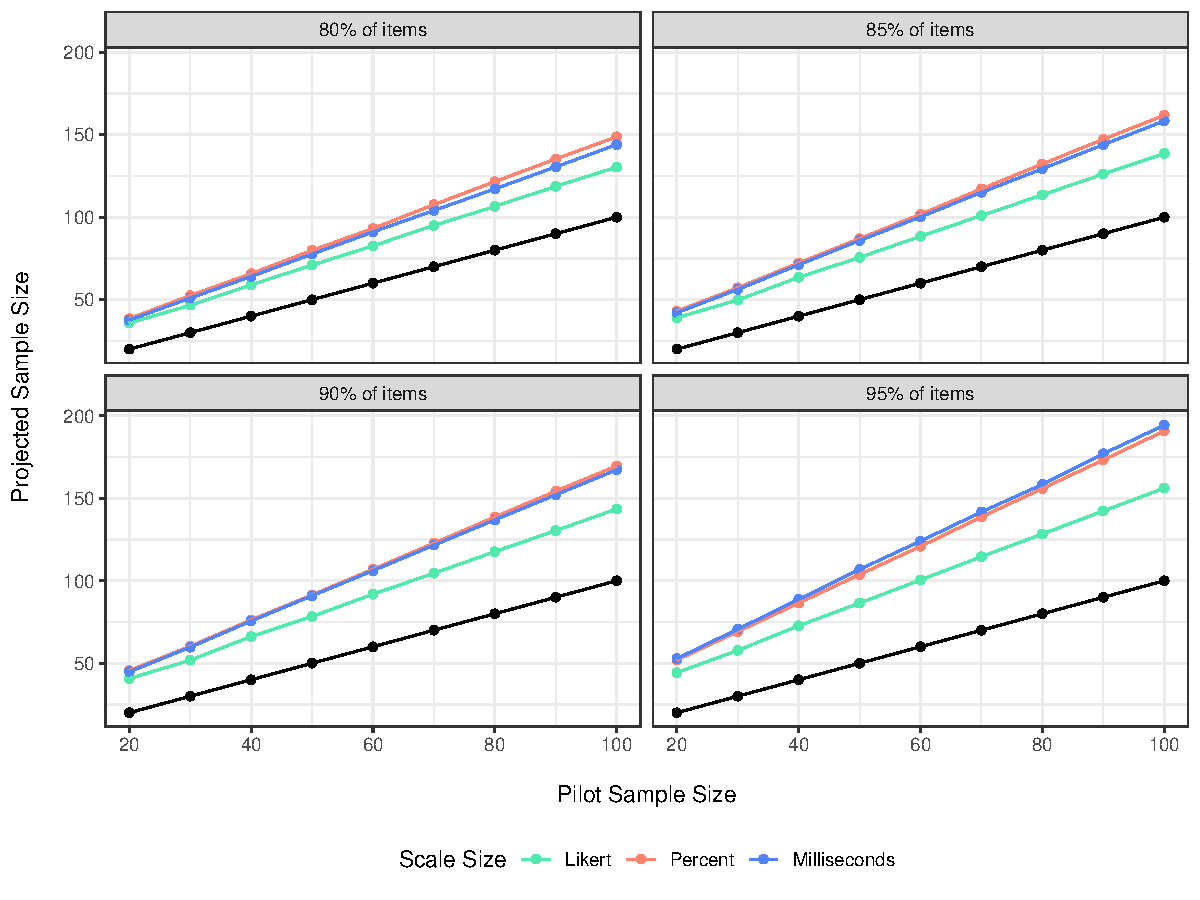
\includegraphics[keepaspectratio]{manuscript_draft_files/figure-latex/scale-size-figure-1.pdf}}
\caption{\label{fig:scale-size-figure}Simulated pilot sample size and final projected sample size to achieve 80\%, 85\%, 90\%, and 95\% of items below threshold. These values are averaged over all other variables including decile. Black dots represent original sample size for reference.}
\end{figure}

Figure \ref{fig:scale-size-figure} demonstrates the influence of scale size on the results separated by potential cutoff decile level. The black dots denote the original sample size for reference. Larger scales have more potential variability, and therefore, we see that percent and millisecond scales project a larger required sample size. This relationship does not appear to be linear with scale size, as percent scales often represent the highest projected sample size. Potentially, this finding is due to the larger proportion of possible variance -- the variance of the item standard deviations / total possible variance -- was largest for percent scales in this set of simulations (\(p_{Percent}\) = .13). This finding may be an interaction with heterogeneity, as the Likert scale had the next highest percent variability in item standard errors (\(p_{Likert}\) = .10), followed by milliseconds (\(p_{Milliseconds}\) = .06).

\subsubsection{Skew}\label{skew}

\begin{figure}
\centering
\pandocbounded{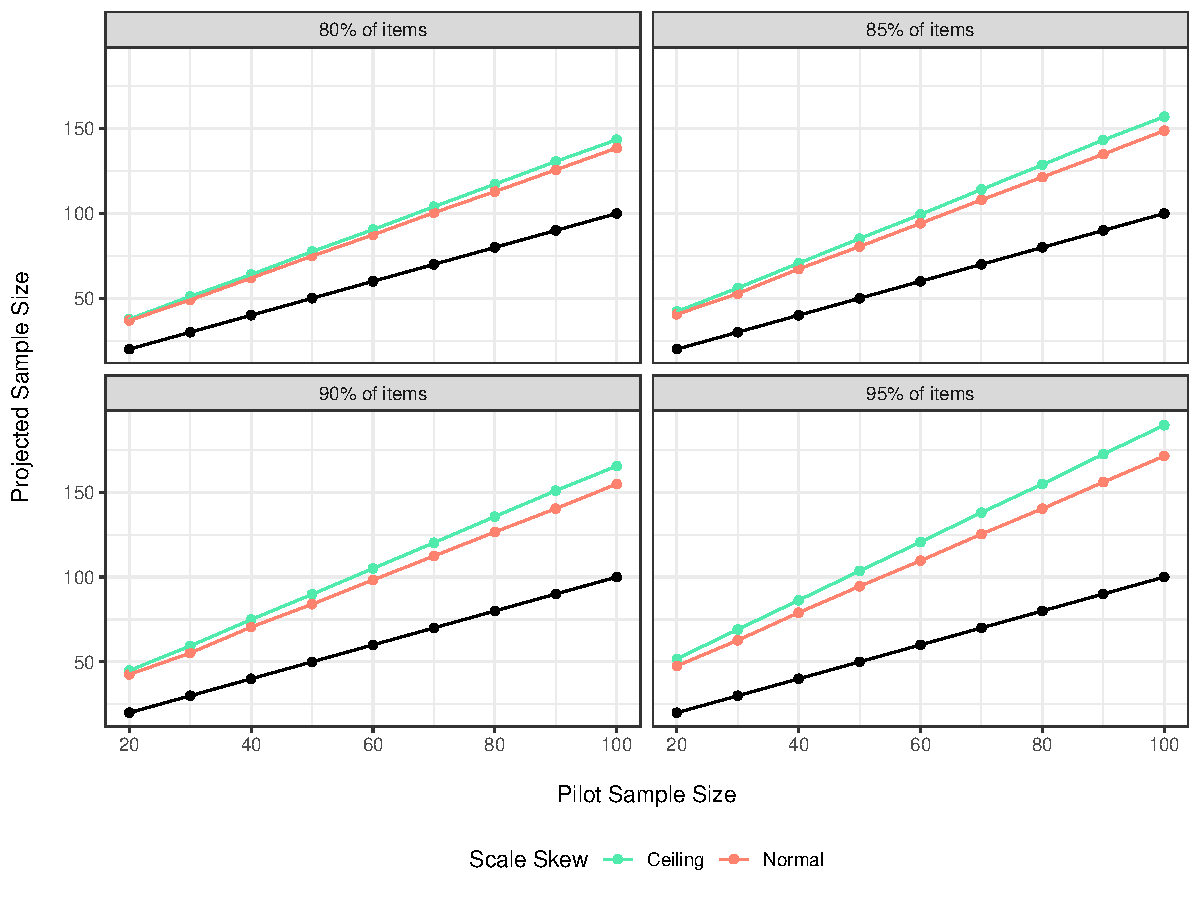
\includegraphics[keepaspectratio]{manuscript_draft_files/figure-latex/scale-skew-figure-1.pdf}}
\caption{\label{fig:scale-skew-figure}Simulated pilot sample size and final projected sample size to achieve 80\%, 85\%, 90\%, and 95\% of items below threshold. In comparison to Figure 1, this figure shows projected sample size for ceiling versus symmetric distributions on each scale. All other variables are averaged together, and black dots represent original sample size for reference.}
\end{figure}

Figure \ref{fig:scale-skew-figure} displays that ceiling distributions, averaged over all other variables, show slightly higher estimates than symmetric distributions. This result is consistent across scale type and heterogeneity, as results indicated that they are often the same or slightly higher for ceiling distributions.

\subsubsection{Item Heterogeneity}\label{item-heterogeneity}

\begin{figure}
\centering
\pandocbounded{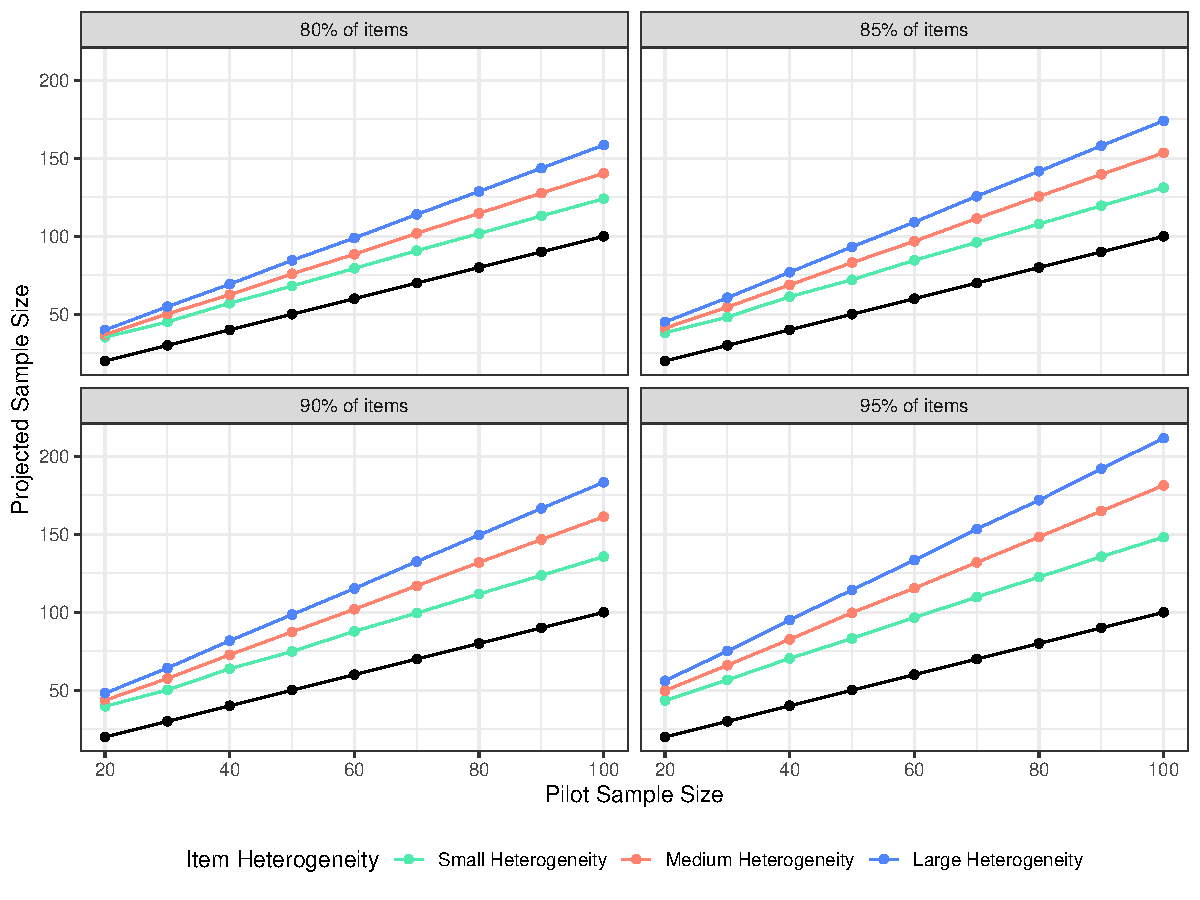
\includegraphics[keepaspectratio]{manuscript_draft_files/figure-latex/scale-hetero-figure-1.pdf}}
\caption{\label{fig:scale-hetero-figure}Simulated pilot sample size and final projected sample size to achieve 80\%, 85\%, 90\%, and 95\% of items below threshold. In comparison to Figure 1 and 2, this figure shows projected sample size or differing amounts of heterogeneity on each scale. All other variables are averaged together, and black dots represent original sample size for reference.}
\end{figure}

Figure \ref{fig:scale-hetero-figure} displays the results for item heterogeneity for different levels of potential power. In this figure, we found that our suggested procedure does capture the differences in heterogeneity. As heterogeneity increases in item variances, the proposed sample size also increases.

\begin{table}[tbp]

\begin{center}
\begin{threeparttable}

\caption{\label{tab:table-predict-largest}Prediction of Proposed Sample Size from Simulated Variables}

\begin{tabular}{llllll}
\toprule
Term & Estimate & $SE$ & $t$ & $p$ & $pr^2$\\
\midrule
Intercept & -27.30 & 3.08 & -8.87 & < .001 & .335\\
Pilot Sample Size & 1.51 & 0.03 & 54.76 & < .001 & .951\\
Scale: Likert v Percent & 7.00 & 1.80 & 3.89 & < .001 & .088\\
Scale: Likert v Milllisecond & 25.63 & 1.87 & 13.74 & < .001 & .548\\
Proportion Variability & 312.44 & 19.86 & 15.73 & < .001 & .613\\
Data: Ceiling v Symmetric & -7.16 & 1.41 & -5.08 & < .001 & .142\\
\bottomrule
\end{tabular}

\end{threeparttable}
\end{center}

\end{table}

Using a regression model, we predicted proposed sample size using pilot sample size, scale size, proportion variability (i.e., heterogeneity), and data type (symmetric, ceiling). As shown in Table \ref{tab:table-predict-largest}, the largest influence on proposed sample size is the original pilot sample size, followed by proportion of variance/heterogeneity, and then data and scale sizes.

\subsection{Projected Sample Size Sensitivity to Pilot Sample Size}\label{projected-sample-size-sensitivity-to-pilot-sample-size}

In our second question, we examined if the suggested procedure was sensitive to the amount of information present in the pilot data. Larger pilot data is more informative, and therefore, we should expect a lower projected sample size. As shown in each figure presented already, we do not find this effect. These simulations from the pilot data would nearly always suggest a larger sample size - mostly in a linear trend increasing with sample sizes. This result comes from the nature of the procedure - if we base our estimates on a SE cutoff, we will almost always need a bit more people for items to meet those goals. This result does not achieve our second goal.

Therefore, we suggest using a correction factor on the simulation procedure to account for the known asymptotic nature of power (i.e., at larger sample sizes power increases level off). For this function in our simulation study, we combined a correction factor for upward biasing of effect sizes (Hedges' correction) with the formula for exponential decay calculations. The decay factor was calculated as follows:

\[ 1 - \sqrt{\frac{N_{Pilot} - min(N_{Simulation})}{N_{Pilot}}}^{log_2(N_{Pilot})}\]

\(N_{Pilot}\) indicates the sample size of the pilot data minus the minimum simulated sample size to ensure that the smallest sample sizes do not decay (i.e., the formula zeroes out). This value is raised to the power of \(log_2\) of the sample size of the pilot data, which decreases the impact of the decay to smaller increments for increasing sample sizes. This value is then multiplied by the projected sample size. As shown in Figure \ref{fig:corrected-figure}, this correction factor produces the desired quality of maintaining that small pilot studies should \emph{increase} sample size, and that sample size suggestions level off as pilot study data sample size increases.

\begin{figure}
\centering
\pandocbounded{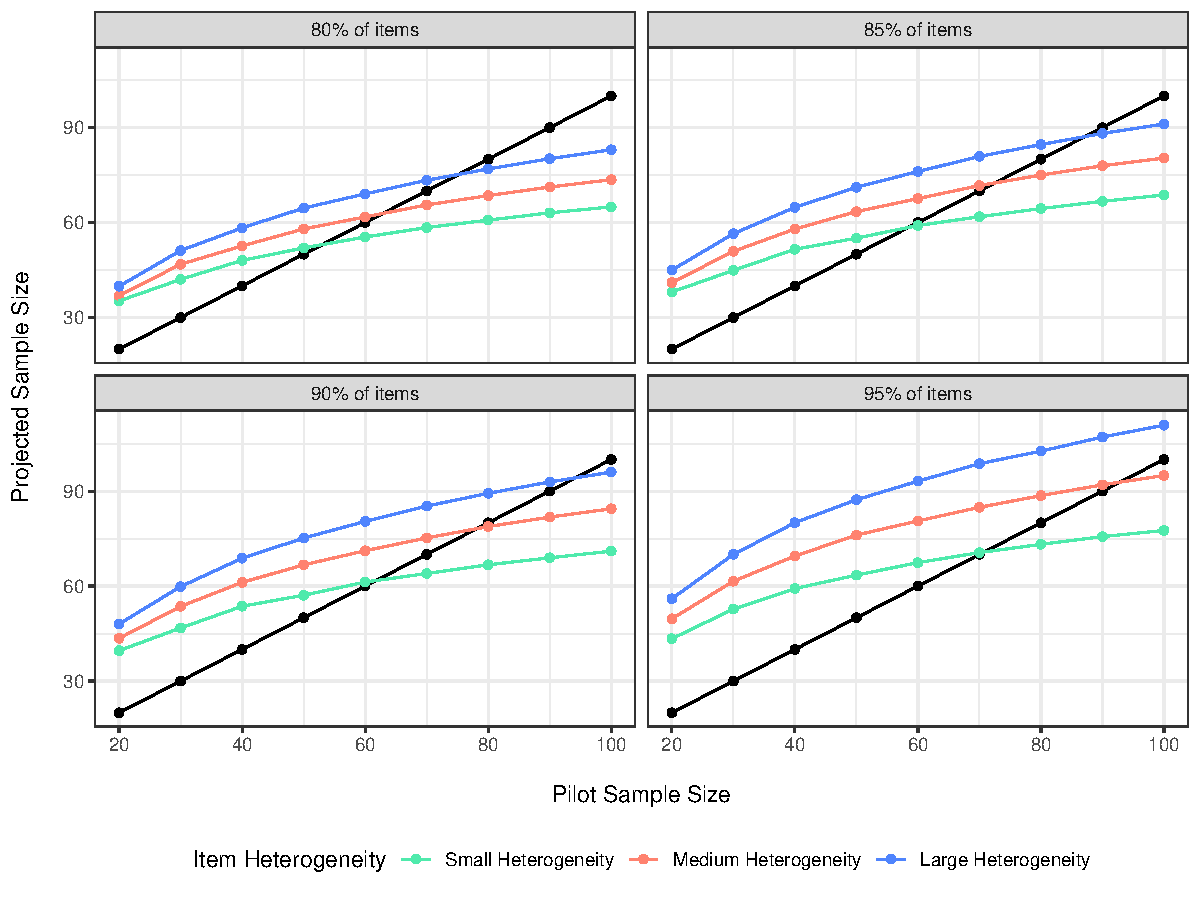
\includegraphics[keepaspectratio]{manuscript_draft_files/figure-latex/corrected-figure-1.pdf}}
\caption{\label{fig:corrected-figure}Corrected projected sample sizes for variability and power levels to achieve 80\%, 85\%, 90\%, and 95\% of items below threshold. All other variables are averaged together, and black dots represent original sample size for reference.}
\end{figure}

\subsection{Corrections for Individual Researchers}\label{corrections-for-individual-researchers}

We have portrayed that this procedure, with a correction factor, can perform as desired. However, within real scenarios, researchers will only have one pilot sample, not the various simulated samples shown above. What should the researcher do to correct their projected sample size from their own pilot data simulations?

To explore if we could recover the corrected sample size from data a researcher would have, we used regression models to create a formula for researcher correction. The researcher employing our procedure would have the possible following variables from their simulations on their (one) pilot dataset: 1) proposed sample size, 2) pilot sample size, 3) estimate of heterogeneity for the items, 4) and the estimated percent of items below the threshold. Given the non-linear nature of the correction, we added each variable and its non-linear \texttt{log2} transform to the regression equation, as this function was used to create the correction. The intercept only model was used as a starting point (i.e., \texttt{corrected\ sample\ \textasciitilde{}\ 1}), and then all eight variables (each variable and their \texttt{log2} transform) were entered into the regression equation.

As shown in Table \ref{tab:table-correction}, all variables were significant predictors of the new sample size. Proposed sample size and original sample size were the largest predictors -- unsurprising given the correction formula employed -- followed by the percent ``power'' level and proportion of variance. This formula approximation captures \(R^2 = .99\), 90\% CI \([0.99, 0.99]\) of the variance in sample size scores and should allow a researcher to estimate based on their own data, \(F(8, 4527) = 67,497.54\), \(p < .001\). We provide convenience functions in our additional materials to assist researchers in estimating the final corrected sample size.

\begin{table}[tbp]

\begin{center}
\begin{threeparttable}

\caption{\label{tab:table-correction}Parameters for All Decile Cutoff Scores}

\begin{tabular}{lllll}
\toprule
Term & Estimate & $SE$ & $t$ & $p$\\
\midrule
Intercept & 111.049 & 78.248 & 1.419 & .156\\
Projected Sample Size & 0.429 & 0.002 & 185.360 & < .001\\
Pilot Sample Size & 15.434 & 3.617 & 4.267 & < .001\\
Log2 Projected Sample Size & -0.718 & 0.007 & -103.787 & < .001\\
Log2 Pilot Sample Size & 0.606 & 0.259 & 2.343 & .019\\
Log2 Power & 19.522 & 0.215 & 90.693 & < .001\\
Proportion Variability & -0.729 & 0.232 & -3.143 & .002\\
Log2 Proportion Variability & 4.655 & 0.269 & 17.296 & < .001\\
Power & -39.367 & 15.640 & -2.517 & .012\\
\bottomrule
\end{tabular}

\end{threeparttable}
\end{center}

\end{table}

\subsection{Choosing an Appropriate cutoff}\label{choosing-an-appropriate-cutoff}

Last, we examined the question of an appropriate SE decile. First, the 0, 1st, and 2nd deciles are likely too restrictive, providing very large estimates that do not always find a reasonable sample size in proportion to the pilot sample size, scale size, and heterogeneity. If we examine the \(R^2\) values for each decile of our regression equation separately, we find that the values are all \(R^2\) \textgreater{} .99 with very little differences between them. Figures \ref{fig:decile40-figure} and \ref{fig:decile50-figure} illustrate the corrected scores for simulations at the 4th and 5th decile recommended cutoff for item standard errors. For small heterogeneity, differences in decile are minimal, while larger heterogeneity shows more correction at the 4th decile range, especially for scales with larger potential variance. Therefore, we would suggest the 4th decile to overpower each item for Step 2.

\begin{figure}
\centering
\pandocbounded{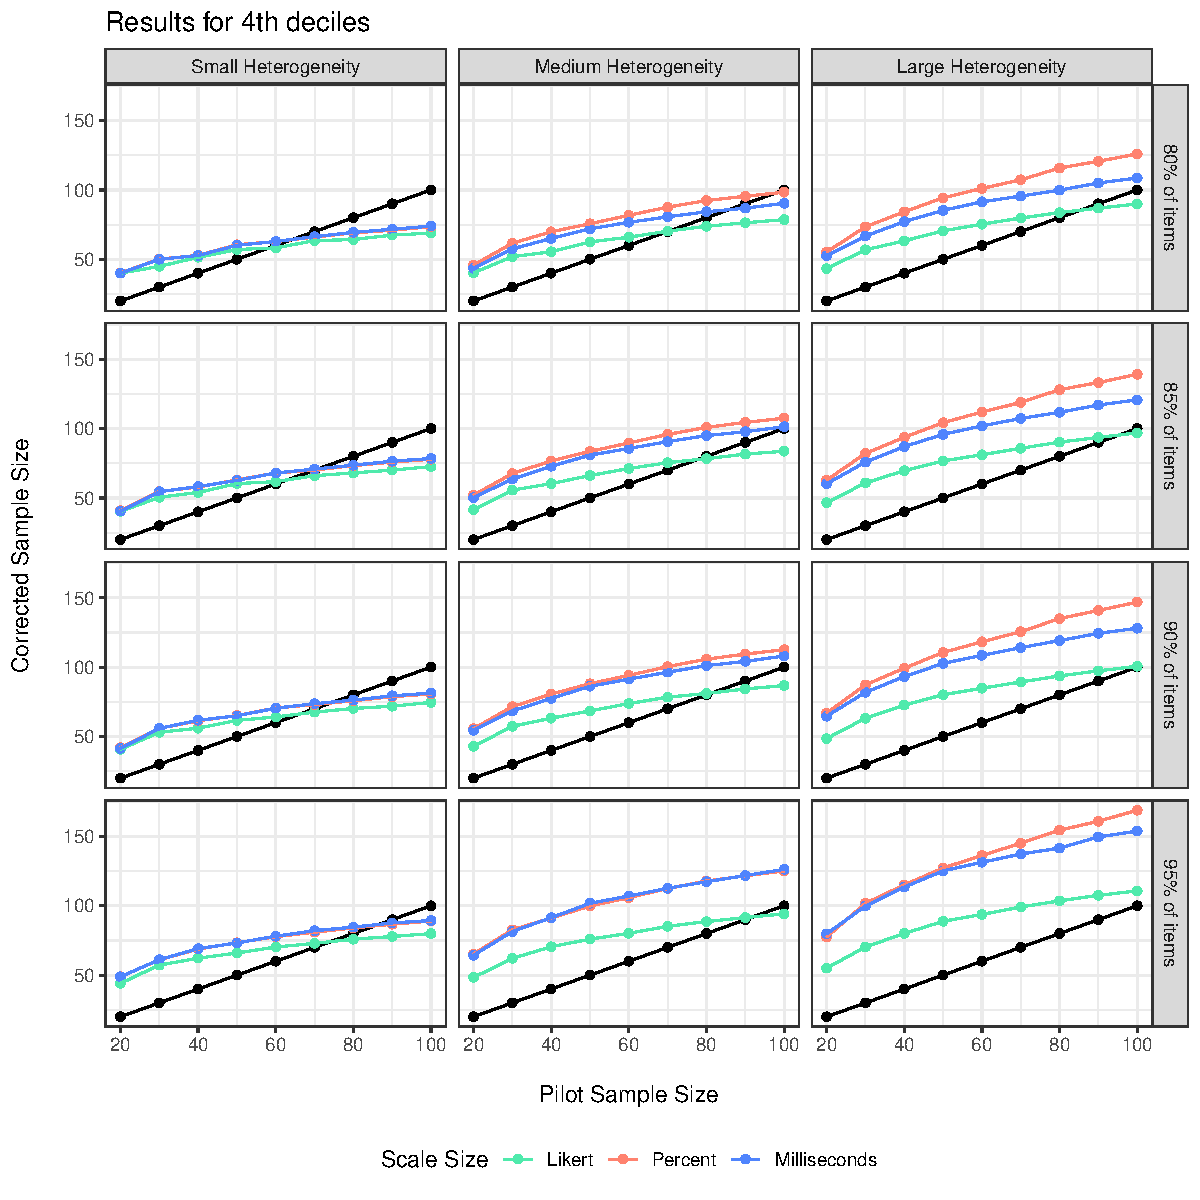
\includegraphics[keepaspectratio]{manuscript_draft_files/figure-latex/decile40-figure-1.pdf}}
\caption{\label{fig:decile40-figure}Comparison of the cutoffs for 4th deciles across heterogeneity (columns), powering of items (rows), and scale size (color).}
\end{figure}

\begin{figure}
\centering
\pandocbounded{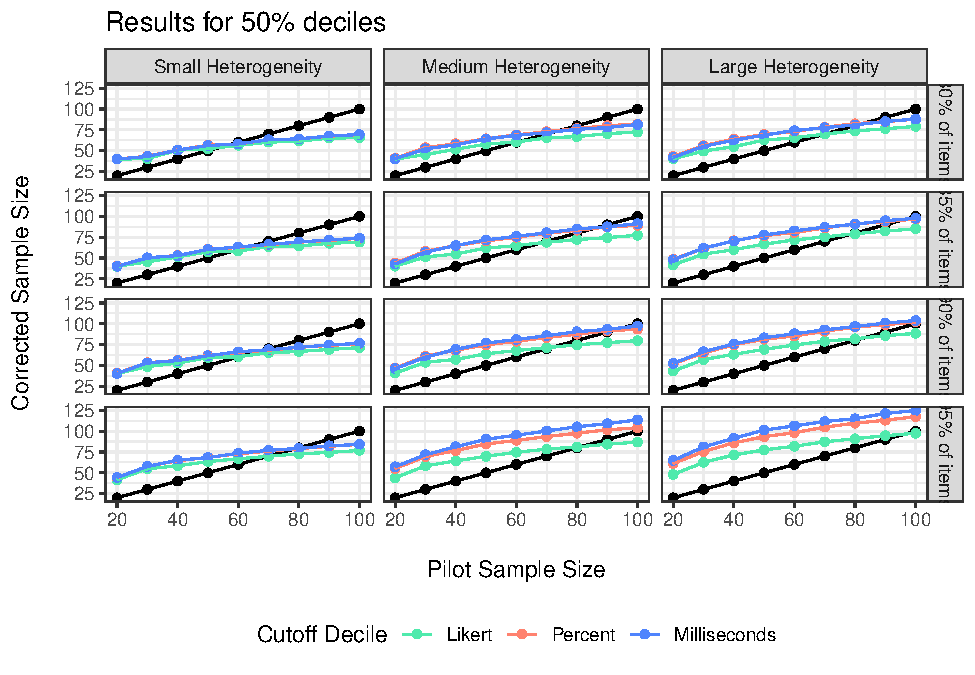
\includegraphics[keepaspectratio]{manuscript_draft_files/figure-latex/decile50-figure-1.pdf}}
\caption{\label{fig:decile50-figure}Comparison of the cutoffs for 5th deciles across heterogeneity (columns), powering of items (rows), and scale size (color).}
\end{figure}

The final formula for 4th decile correction is provided in Table \ref{tab:table-decile}. Proportion of variance can be calculated with the following:

\[\frac{SD_{Item SD}}{\sqrt{\frac{(Maximum - Minimum)^2}{4}}}\] where maximum and minimum are the max and min values found in the scale (or the data, if the scale is unbounded). This formula would be applied in Step 5 of the proposed procedure. While the estimated coefficients could change given variations on our simulation parameters, the general size and pattern of coefficients was consistent, and therefore, we believe this correction equation should work for a variety of use cases. We will now demonstrate the final procedure on the example provided earlier.

\begin{table}[tbp]

\begin{center}
\begin{threeparttable}

\caption{\label{tab:table-decile}Parameters for 4th decile Cutoff Scores}

\begin{tabular}{lllll}
\toprule
Term & Estimate & $SE$ & $t$ & $p$\\
\midrule
Intercept & 206.589 & 128.861 & 1.603 & .109\\
Projected Sample Size & 0.368 & 0.005 & 71.269 & < .001\\
Pilot Sample Size & -0.770 & 0.013 & -59.393 & < .001\\
Log2 Projected Sample Size & 27.541 & 0.552 & 49.883 & < .001\\
Log2 Pilot Sample Size & 2.583 & 0.547 & 4.725 & < .001\\
Log2 Power & -66.151 & 25.760 & -2.568 & .010\\
Proportion Variability & 16.405 & 6.005 & 2.732 & .006\\
Log2 Proportion Variability & -1.367 & 0.382 & -3.577 & < .001\\
Power & 1.088 & 0.426 & 2.552 & .011\\
\bottomrule
\end{tabular}

\end{threeparttable}
\end{center}

\end{table}

\section{Updated Example}\label{updated-example}

\begin{lltable}

\begin{TableNotes}[para]
\normalsize{\textit{Note.} SS = Sample Size, Proj = Projected, Prop = Proportion, Var = Variance, Cor = Corrected}
\end{TableNotes}

\scriptsize{

\begin{longtable}{llllllllllll}\noalign{\getlongtablewidth\global\LTcapwidth=\longtablewidth}
\caption{\label{tab:table-scores-updated}Applied Correction for Each Proposed Sample Size}\\
\toprule
Formula & Intercept & Proj SS & Pilot SS & Log Proj SS & Log Pilot SS & Log Power & Prop Var & Log Prop Var & Power & Loss & Cor SS\\
\midrule
\endfirsthead
\caption*{\normalfont{Table \ref{tab:table-scores-updated} continued}}\\
\toprule
Formula & Intercept & Proj SS & Pilot SS & Log Proj SS & Log Pilot SS & Log Power & Prop Var & Log Prop Var & Power & Loss & Cor SS\\
\midrule
\endhead
Formula & 206.59 & 0.37 & -0.77 & 27.54 & 2.58 & -66.15 & 16.40 & -1.37 & 1.09 & NA & NA\\
Concrete 80 & 1.00 & 45.00 & 29.00 & 5.49 & 4.86 & 6.32 & 0.14 & -2.82 & 80.00 & 39.63 & 42.56\\
Concrete 85 & 1.00 & 45.00 & 29.00 & 5.49 & 4.86 & 6.41 & 0.14 & -2.82 & 85.00 & 39.29 & 42.19\\
Concrete 90 & 1.00 & 50.00 & 29.00 & 5.64 & 4.86 & 6.49 & 0.14 & -2.82 & 90.00 & 45.30 & 48.65\\
Concrete 95 & 1.00 & 55.00 & 29.00 & 5.78 & 4.86 & 6.57 & 0.14 & -2.82 & 95.00 & 51.21 & 54.99\\
LDT 80 & 1.00 & 60.00 & 33.00 & 5.91 & 5.04 & 6.32 & 0.08 & -3.60 & 80.00 & 54.08 & 67.68\\
LDT 85 & 1.00 & 75.00 & 33.00 & 6.23 & 5.04 & 6.41 & 0.08 & -3.60 & 85.00 & 68.12 & 85.25\\
LDT 90 & 1.00 & 90.00 & 33.00 & 6.49 & 5.04 & 6.49 & 0.08 & -3.60 & 90.00 & 80.87 & 101.20\\
LDT 95 & 1.00 & 125.00 & 33.00 & 6.97 & 5.04 & 6.57 & 0.08 & -3.60 & 95.00 & 107.09 & 134.00\\
\bottomrule
\addlinespace
\insertTableNotes
\end{longtable}

}

\end{lltable}

The updated proposal steps are in Table \ref{tab:table-summary} on the right hand side. The main change occurs in Step 2 with a designated cutoff decile, and Step 5 with a correction score. Using the data from the 4th decile in Table \ref{tab:table-example}, we can determine that the stopping rule SE for concreteness ratings would be 0.18, and the stopping rule SE for lexical decision times would be 56.93. For Step 5, we apply our correction formula separately for each one, as they have different variability scores, and these scores are shown in Table \ref{tab:table-scores-updated}. Each row was multiplied by row one's formula, and then these scores are summed for the final corrected sample size. Sample sizes cannot be proportional, so we recommend rounding up to the nearest whole number.

For one additional consideration, we calculated the potential amount of data retention given that participants could indicate they did not know a word (\(M_{answered}\) = 0.93, \emph{SD} = 0.11) in the concreteness task or answer a trial incorrectly in the lexical decision task (\(M_{correct}\) = 0.80, \emph{SD} = 0.21). In order to account for this data loss, the potential sample sizes were multiplied by \(\frac{1}{p_{retained}}\) where the denominator is proportion retained for each task.

\section{Additional Materials}\label{additional-materials}

\subsection{Package}\label{package}

We have developed functions to implement the suggested procedure as part of a semantic priming focused package \texttt{semanticprimeR}. You can install the package from GitHub using: \texttt{devtools::install\_github("SemanticPriming/semanticprimeR")}. We detail the functions below with proposed steps in the process.

\emph{Step 1}. Ideally, researchers would have pilot data that represented their proposed data collection. This data should be formatted in long format wherein each row represents the score from an item by participant, rather than wide format wherein each column represents an item and each row represents a single participant. The \texttt{tidyr::pivot\_longer()} or \texttt{reshape::melt()} functions can be used to reformat wide data. If no pilot data is available, the \texttt{simulate\_population()} function can be used with the following arguments (and example numbers, * indicates optional). This function will return a dataframe with the simulated normal values for each item.

\begin{Shaded}
\begin{Highlighting}[]
\CommentTok{\# devtools::install\_github("SemanticPriming/semanticprimeR")}
\FunctionTok{library}\NormalTok{(semanticprimeR)}
\NormalTok{pops }\OtherTok{\textless{}{-}} \FunctionTok{simulate\_population}\NormalTok{(}\AttributeTok{mu =} \DecValTok{4}\NormalTok{, }\CommentTok{\# item means}
  \AttributeTok{mu\_sigma =}\NormalTok{ .}\DecValTok{2}\NormalTok{, }\CommentTok{\# variability in item means }
  \AttributeTok{sigma =} \DecValTok{2}\NormalTok{, }\CommentTok{\# item standard deviations}
  \AttributeTok{sigma\_sigma =}\NormalTok{ .}\DecValTok{2}\NormalTok{, }\CommentTok{\# standard deviation of the standard deviations}
  \AttributeTok{number\_items =} \DecValTok{30}\NormalTok{, }\CommentTok{\# number of items}
  \AttributeTok{number\_scores =} \DecValTok{20}\NormalTok{, }\CommentTok{\# number of participants}
  \AttributeTok{smallest\_sigma =}\NormalTok{ .}\DecValTok{02}\NormalTok{, }\CommentTok{\#* smallest possible standard deviation}
  \AttributeTok{min\_score =} \DecValTok{1}\NormalTok{, }\CommentTok{\#* minimum score for truncating purposes}
  \AttributeTok{max\_score =} \DecValTok{7}\NormalTok{, }\CommentTok{\#* maximum score for truncating purposes}
  \AttributeTok{digits =} \DecValTok{0}\NormalTok{) }\CommentTok{\#* number of digits for rounding}
  
\FunctionTok{head}\NormalTok{(pops)}
\end{Highlighting}
\end{Shaded}

\begin{verbatim}
##   item score
## 1    1     3
## 2    2     5
## 3    3     6
## 4    4     5
## 5    5     5
## 6    6     7
\end{verbatim}

\emph{Step 2}. In step 2, we can use \texttt{calculate\_cutoff()} to calculate the standard error of the items, the standard deviation of the standard errors and the corresponding proportion of variance possible, and the 4th decile cutoff score. The \texttt{pops} dataframe can be used in this function, which has columns named \texttt{item} for the item labels (i.e., 1, 2, 3, 4 or characters can be used), and \texttt{score} for the dependent variable. This function returns a list of values to be used in subsequent steps.

\begin{Shaded}
\begin{Highlighting}[]
\NormalTok{cutoff }\OtherTok{\textless{}{-}} \FunctionTok{calculate\_cutoff}\NormalTok{(}\AttributeTok{population =}\NormalTok{ pops, }\CommentTok{\# pilot data or simulated data}
  \AttributeTok{grouping\_items =} \StringTok{"item"}\NormalTok{, }\CommentTok{\# name of the item indicator column}
  \AttributeTok{score =} \StringTok{"score"}\NormalTok{, }\CommentTok{\# name of the dependent variable column}
  \AttributeTok{minimum =} \DecValTok{1}\NormalTok{, }\CommentTok{\# minimum possible/found score}
  \AttributeTok{maximum =} \DecValTok{7}\NormalTok{) }\CommentTok{\# maximum possible/found score}
                           
\NormalTok{cutoff}\SpecialCharTok{$}\NormalTok{se\_items }\CommentTok{\# all standard errors of items}
\end{Highlighting}
\end{Shaded}

\begin{verbatim}
##  [1] 0.4285840 0.3618301 0.3561490 0.3211820 0.3938675 0.3661679 0.4679181
##  [8] 0.2643264 0.3524351 0.2663101 0.4772454 0.4222434 0.4369451 0.4173853
## [15] 0.3266658 0.3871284 0.3802700 0.3913539 0.4701623 0.3802700 0.4142209
## [22] 0.3441236 0.3732856 0.4032761 0.4013136 0.3515005 0.3647277 0.3966969
## [29] 0.3925289 0.3598245
\end{verbatim}

\begin{Shaded}
\begin{Highlighting}[]
\NormalTok{cutoff}\SpecialCharTok{$}\NormalTok{sd\_items }\CommentTok{\# standard deviation of the standard errors}
\end{Highlighting}
\end{Shaded}

\begin{verbatim}
## [1] 0.05056835
\end{verbatim}

\begin{Shaded}
\begin{Highlighting}[]
\NormalTok{cutoff}\SpecialCharTok{$}\NormalTok{cutoff }\CommentTok{\# 4th decile score}
\end{Highlighting}
\end{Shaded}

\begin{verbatim}
##       40% 
## 0.3704385
\end{verbatim}

\begin{Shaded}
\begin{Highlighting}[]
\NormalTok{cutoff}\SpecialCharTok{$}\NormalTok{prop\_var }\CommentTok{\# proportion of possible variance }
\end{Highlighting}
\end{Shaded}

\begin{verbatim}
## [1] 0.01685612
\end{verbatim}

\emph{Step 3}. The \texttt{simulate\_samples()} function creates simulated samples from the pilot or simulated population data to estimate the number of participants needed for item standard error to be below the cutoff calculated in Step 2. This function returns a list of samples with sizes that start at the \texttt{start} size, increase by \texttt{increase}, and end with the \texttt{stop} sample size. The population or pilot data will be included in \texttt{population}, and the item column indicator should be included in \texttt{grouping\_items}. The \texttt{nsim} argument determines the number of simulations to run.

\begin{Shaded}
\begin{Highlighting}[]
\NormalTok{samples }\OtherTok{\textless{}{-}} \FunctionTok{simulate\_samples}\NormalTok{(}\AttributeTok{start =} \DecValTok{20}\NormalTok{, }\CommentTok{\# starting sample size}
  \AttributeTok{stop =} \DecValTok{100}\NormalTok{, }\CommentTok{\# stopping sample size}
  \AttributeTok{increase =} \DecValTok{5}\NormalTok{, }\CommentTok{\# increase simulated samples by this amount}
  \AttributeTok{population =}\NormalTok{ pops, }\CommentTok{\# population or pilot data}
  \AttributeTok{replace =} \ConstantTok{TRUE}\NormalTok{, }\CommentTok{\# simulate with replacement? }
  \AttributeTok{nsim =} \DecValTok{500}\NormalTok{, }\CommentTok{\# number of simulations to run}
  \AttributeTok{grouping\_items =} \StringTok{"item"}\NormalTok{) }\CommentTok{\# item column label  }

\FunctionTok{head}\NormalTok{(samples[[}\DecValTok{1}\NormalTok{]])}
\end{Highlighting}
\end{Shaded}

\begin{verbatim}
## # A tibble: 6 x 2
## # Groups:   item [1]
##    item score
##   <int> <dbl>
## 1     1     3
## 2     1     4
## 3     1     3
## 4     1     4
## 5     1     4
## 6     1     4
\end{verbatim}

\emph{Step 4 and 5}. The proportion of simulated items across sample sizes below the cutoff score can then be calculated using \texttt{calculate\_proportion()}. This function returns a dataframe including each sample size with the proportion of items below that cutoff to use in the next function. The \texttt{samples} and \texttt{cutoff} arguments were previously calculated with our functions. The column for item labels and dependent variables are included as \texttt{grouping\_items} and \texttt{score} arguments to ensure the right calculations.

\begin{Shaded}
\begin{Highlighting}[]
\NormalTok{proportion\_summary }\OtherTok{\textless{}{-}} \FunctionTok{calculate\_proportion}\NormalTok{(}\AttributeTok{samples =}\NormalTok{ samples, }\CommentTok{\# samples list}
  \AttributeTok{cutoff =}\NormalTok{ cutoff}\SpecialCharTok{$}\NormalTok{cutoff, }\CommentTok{\# cut off score }
  \AttributeTok{grouping\_items =} \StringTok{"item"}\NormalTok{, }\CommentTok{\# item column name}
  \AttributeTok{score =} \StringTok{"score"}\NormalTok{) }\CommentTok{\# dependent variable column name }

\FunctionTok{head}\NormalTok{(proportion\_summary)}
\end{Highlighting}
\end{Shaded}

\begin{verbatim}
## # A tibble: 6 x 2
##   percent_below sample_size
##           <dbl>       <dbl>
## 1         0.4            20
## 2         0.8            25
## 3         0.833          30
## 4         0.967          35
## 5         1              40
## 6         1              45
\end{verbatim}

\emph{Step 6}. Last, we use the \texttt{calculate\_correction()} function to correct the sample size scores given the proposed correction formula. The \texttt{proportion\_summary} from above is used in this function, along with required information about the sample size, proportion of variance from our cutoff calculation, and what power levels should be calculated. Note that the exact percent of items below a cutoff score will be returned if the values in \texttt{power\_levels} are not exactly calculated. The final summary presents the smallest sample size, corrected, for each of the potential power levels.

\begin{Shaded}
\begin{Highlighting}[]
\NormalTok{corrected\_summary }\OtherTok{\textless{}{-}} \FunctionTok{calculate\_correction}\NormalTok{(}
  \AttributeTok{proportion\_summary =}\NormalTok{ proportion\_summary, }\CommentTok{\# prop from above}
  \AttributeTok{pilot\_sample\_size =} \DecValTok{20}\NormalTok{, }\CommentTok{\# number of participants in the pilot data }
  \AttributeTok{proportion\_variability =}\NormalTok{ cutoff}\SpecialCharTok{$}\NormalTok{prop\_var, }\CommentTok{\# proportion variance from cutoff scores}
  \AttributeTok{power\_levels =} \FunctionTok{c}\NormalTok{(}\DecValTok{80}\NormalTok{, }\DecValTok{85}\NormalTok{, }\DecValTok{90}\NormalTok{, }\DecValTok{95}\NormalTok{)) }\CommentTok{\# what levels of power to calculate }

\NormalTok{corrected\_summary}
\end{Highlighting}
\end{Shaded}

\begin{verbatim}
## # A tibble: 4 x 3
##   percent_below sample_size corrected_sample_size
##           <dbl>       <dbl>                 <dbl>
## 1          80            25                  16.6
## 2          96.7          35                  33.7
## 3          96.7          35                  33.7
## 4          96.7          35                  33.7
\end{verbatim}

\subsection{Special Considerations}\label{special-considerations}

\subsubsection{Bimodal Data}\label{bimodal-data}

The above simulations assume symmetric population distributions with small, medium, or large heterogeneity or a skewed distribution with the same heterogeneity. However, as shown in Pollock (2018), sample rating data that appears to have a mean distribution may represent the average two separate distributions (i.e., a bimodal distribution). To examine our procedure with bimodal distributions, we estimated thirty items for three distributions: symmetric, ceiling, and floor distributions for Likert data with small heterogeneity. Bimodal data was created by selecting half of the ceiling distribution and floor distribution to combine together. The number of bimodal items was varied from 0 percent to 100 percent increasing by 10 percent increments for simulated samples. Figure \ref{fig:bimodal-figure} shows an example of 10 of the items within a simulation that estimated that half of the Likert items would be bimodal in nature. The researcher procedure described above was then carried out using \emph{semanticprimeR}.

\begin{figure}
\centering
\pandocbounded{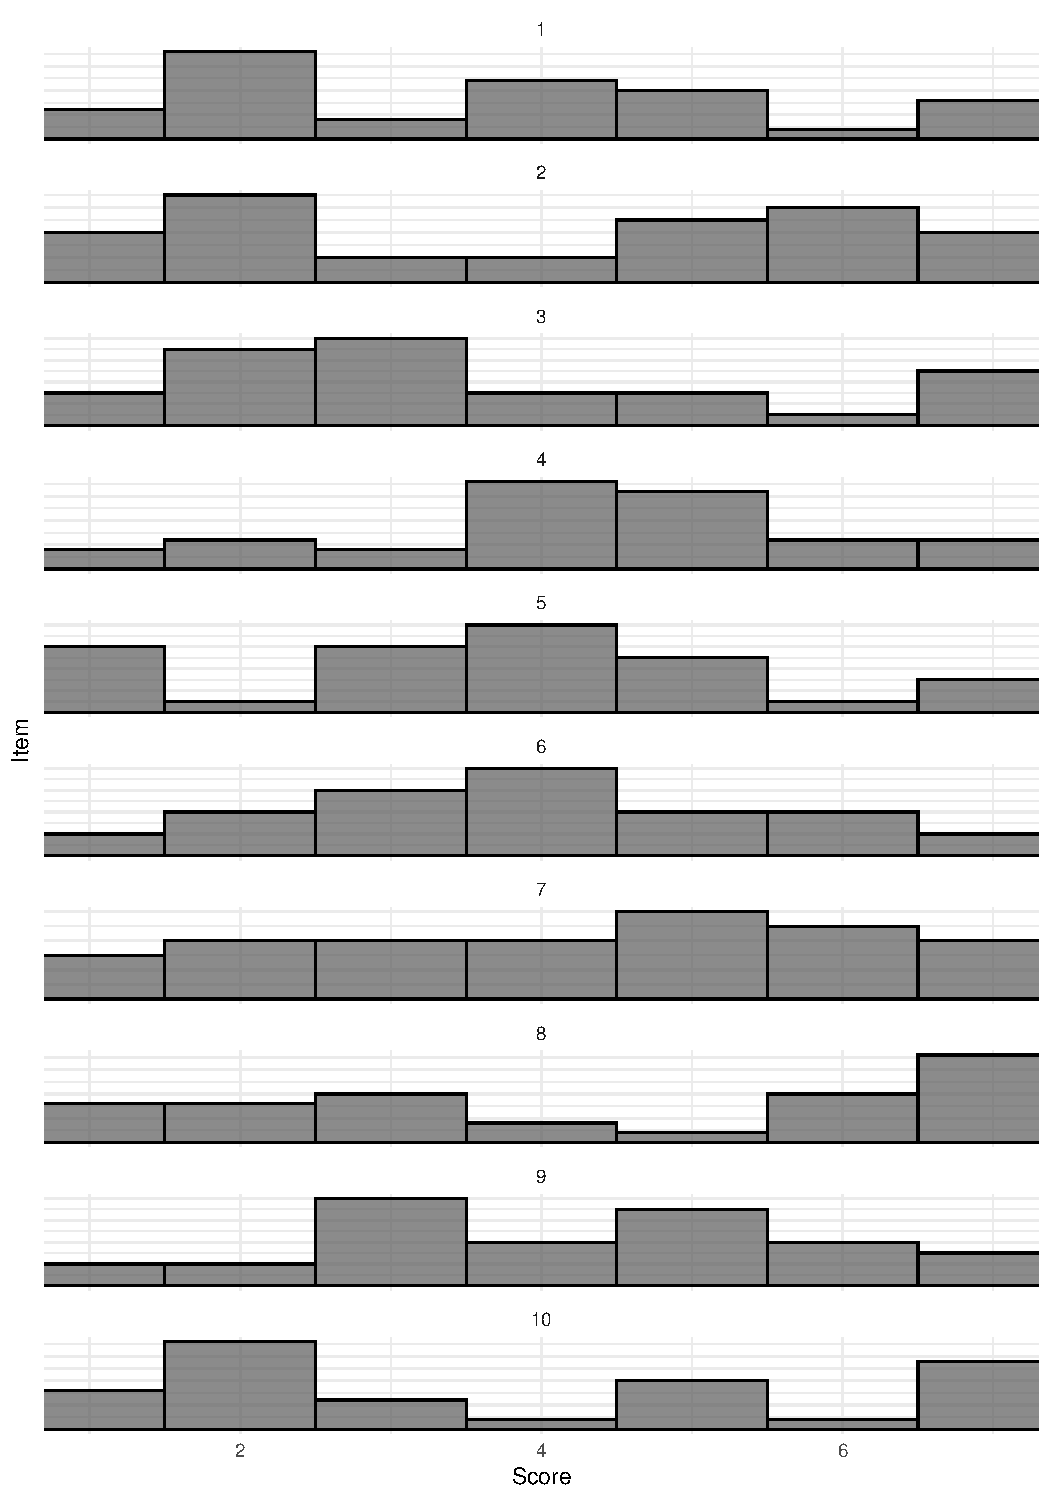
\includegraphics[keepaspectratio]{manuscript_draft_files/figure-latex/bimodal-figure-1.pdf}}
\caption{\label{fig:bimodal-figure}Simulated example of Likert data with half of the items as bimodal distributions.}
\end{figure}

Figure \ref{fig:bimodal-figure} portrays the results of the suggested procedure. The sample with 0 bimodal items demonstrates the same values as above. The proposed sample size increases from 10 to 40\% because of the heterogeneity in SE across items (i.e., with 10\% of items with a larger SE due to their bimodal nature, the required sample size increases). From 50\% to 100\% the sample size decreases because the variance of the SEs across items decreases (i.e., at 100 percent, they are all larger rather than a mix). In theory, these results map onto the conceptual framework - if all items are truly bimodal, we have precisely measured the mean of the bimodal distribution, but this result is likely not the intended result. If researchers expect these distributions (or have representative pilot data), they could examine the data for bimodal items. These items could be estimated separately (i.e., floor effects item 1, ceiling effects item 1) to ensure that both populations of answers are represented in the data.

\begin{figure}
\centering
\pandocbounded{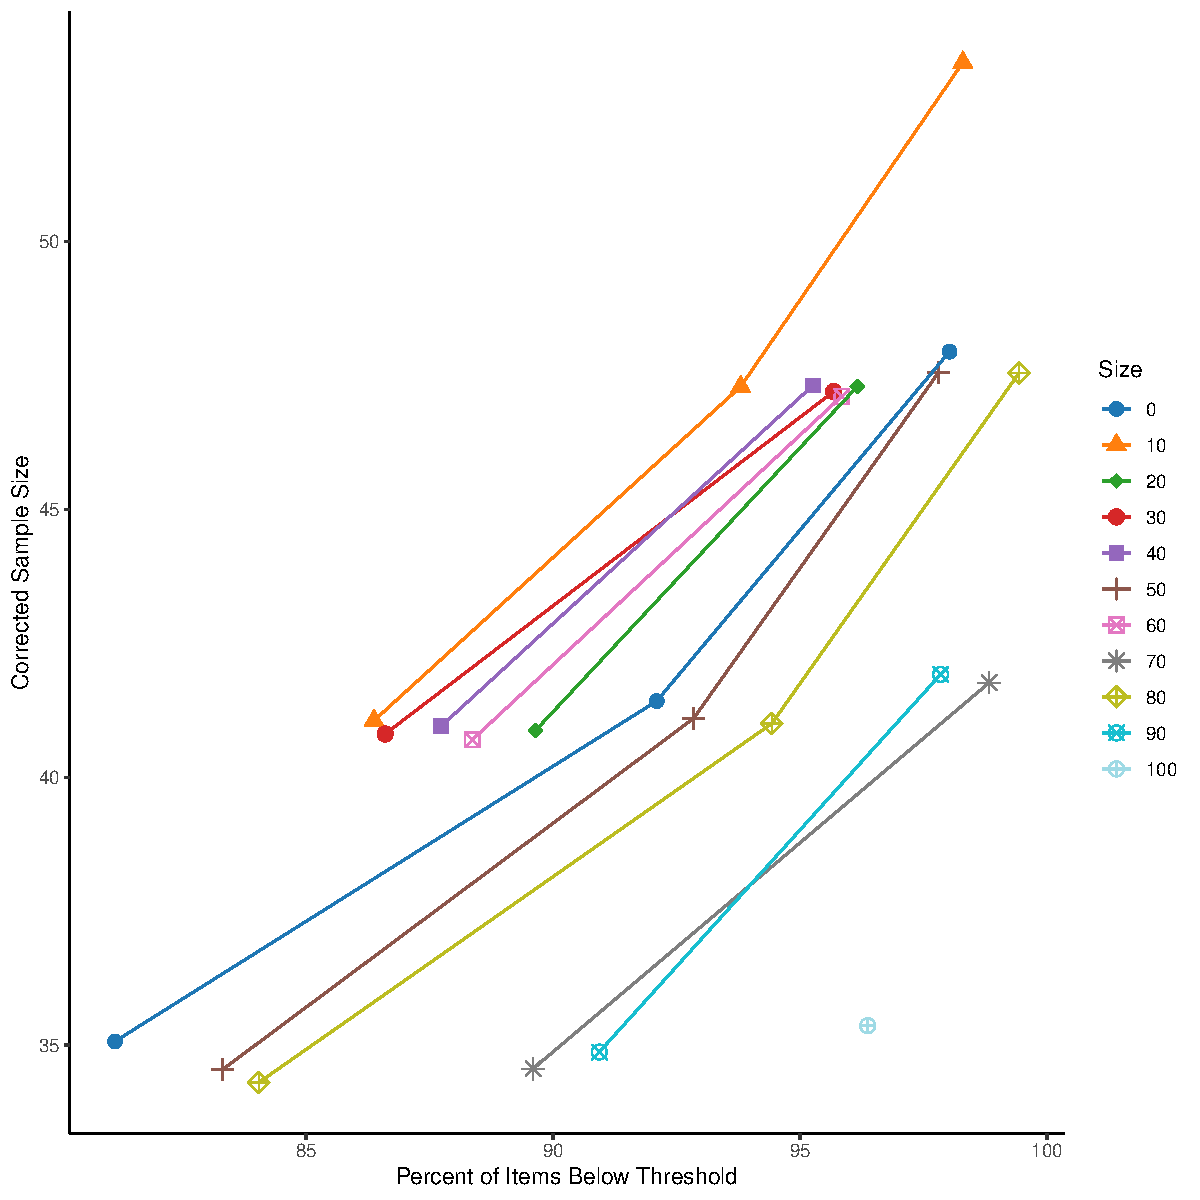
\includegraphics[keepaspectratio]{manuscript_draft_files/figure-latex/bimodal-results-1.pdf}}
\caption{\label{fig:bimodal-results}Estimated sample sizes for distributions that vary in the number of bimodal items. Note that percent below is treated as a continuous factor, and therefore, some estimates are the same (i.e., below 80 and 85 percent may be both estimated as 88\%).}
\end{figure}

\subsubsection{Combining Tools}\label{combining-tools}

Researchers may often be interested in more than just the precision for individual items. The estimation of power via traditional power calculations for a statistical test or the reliability of items could also be of interest for an appropriate dataset for analyses. We would suggest that researchers combine reliability with precision to collect data that are both reliable and precisely measured. For example, one could use our proposed procedure to calculate the sample size for precision. Separately, the researcher would determine the level of reliability they would like to find in items based on previous research or practical guidelines. The minimum sample size could be set based on estimations for hypothesis testing, the stopping rule based on minimum reliability and desired SE for items, and a maximum sample size based on simulations or practical matters. Each data collection represents a unique scenario in which researchers can combine tools based on their needs to collect precise, reliable, and (traditionally defined) adequately powered data. While our proposal may bring to mind the problems with researcher degrees of freedom (Simmons et al., 2011), transparent practices decisions around sample size planning should be encouraged to limit potential questionable research practices.

\subsection{Vignettes}\label{vignettes}

While the example in this manuscript was cognitive linguistics focused, any research using repeated items as a unit of measure could benefit from the proposed newer sampling techniques. Therefore, we provide 12 example vignettes and varied code examples on our OSF page/GitHub site for this manuscript across a range of data types provided by the authors of this manuscript. Examples include psycholinguistics (De Deyne et al., 2008; Heyman et al., 2014; Montefinese et al., 2022), social psychology data (Grahe et al., 2022; Peterson et al., 2022; Ulloa et al., 2014), COVID related data (Montefinese et al., 2021), and cognitive psychology (Barzykowski et al., 2019; Errington et al., 2021; Röer et al., 2013). These can be found on the package tutorial page: \url{https://semanticpriming.github.io/semanticprimeR/}.

\section{Discussion}\label{discussion}

We proposed a method combining AIPE and Monte Carlo simulation to estimate a minimum and maximum sample size and to define a rule for stopping data collection based on narrow confidence intervals on a parameter of interest. In addition, we also demonstrated its practical applications using real-world data. We contend that this procedure is specifically useful for studies with multiple items that intend on using item level focused analyses; furthermore, the utility of measuring each item well can extend to many analysis choices. By focusing on collecting quality data, we can suggest that the data is useful, regardless of the outcome of any hypothesis test.

One limitation of these methods would be our decision to use datasets with very large numbers of items to simulate what might happen within one study. For example, the English Lexicon Project includes thousands of items, and if we were to simulate for all of those, our results would likely suggest needing thousands of participants for most items to reach the criterion. Additionally, as the number of items increases, you may also see very small estimates for sample size due to the correction factor (as with large numbers of items, you could find many items with standard errors below the 4th decile). Therefore, it would be beneficial to consider only simulating what a participant would reasonably complete in a study. Small numbers of repeated items usually result in larger sample sizes proposed from the original pilot data. This result occurs because the smaller number of items means more samples for nearly all to reach the cutoff criteria. These results are similar to what we might expect for a power analysis using a multilevel model - larger numbers of items tend to decrease necessary sample size, while smaller numbers of items tend to increase sample size.

Second, these methods do not ensure the normal interpretation of power, focusing on finding a specific effect for a specific test, \(\alpha\), and so on. As discussed in the introduction, there is not necessarily a one-to-one mapping of hypothesis to analysis; many of the estimations within a traditional power analysis are just that - best approximations for various parameters. These proposed methods and traditional power analysis could be used together to strengthen our understanding of the sample size necessary for both a hypothesis test and a well-tuned estimation. We would advise caution when oversampling (i.e., simulation from data with larger sample sizes than the pilot data) for null-hypothesis power estimates, as these may be upwardly biased in small samples creating Type-I error (Burns et al., 2023).

Researchers should consider this hybrid approach for AIPE and simulation as a powerful tool for hypothesis testing and parameter estimation. This procedure holds benefits for various research studies, specifically replication studies, that usually prioritize subject sample size but rarely item sample size, in spite of the fact that item sample sizes can contribute to power in multilevel models (Brysbaert \& Stevens, 2018; however, see Rouder \& Haaf, 2018 for a discussion of the item-sample size trade off). Replicated effects, accumulated through multiple studies and accurate measurement, contribute to robust meta-analyses, enhancing our understanding of the genuine nature of observed effects. This article helps to achieve this goal by encouraging researchers to conduct studies where the power analysis is not based on the size of the effect but on precise measurement of the stimuli. We argue that this article can be the initial step to apply AIPE in a manner that can allow researchers to use item information to provide a more accurate and statistically reliable measure of the effect we aimed to investigate. In conclusion, item power analysis is a tool to avoid the waste of resources while ensuring that adequately measured items can be achieved. Well measured data can enable us to counteract the literature that contains false positives, allowing us to achieve replicable, high-quality science to establish answers to scientific questions with precision and accuracy.

\section{Open Practices}\label{open-practices}

\begin{itemize}
\tightlist
\item
  Data: All data used in this manuscript and vignettes have been cited and can be found on our repository pages (\url{https://github.com/SemanticPriming/stimuli-power}).
\item
  Analysis Code:

  \begin{itemize}
  \tightlist
  \item
    Manuscript repository with code and data: \url{https://osf.io/swmva/} or \url{https://github.com/SemanticPriming/stimuli-power}
  \item
    Package repository with vignettes and data: \url{https://github.com/SemanticPriming/semanticprimeR}
  \end{itemize}
\item
  Pre-registration: We did not pre-register this study, as it was a simulation study.
\item
  Materials: No materials were used.
\item
  Funding: no funding was provided for this study.
\item
  Conflicts of interest: the researchers declare no conflicts of interest.
\end{itemize}

\newpage

\section{References}\label{references}

\begingroup
\setlength{\parindent}{-0.5in}
\setlength{\leftskip}{0.5in}

\phantomsection\label{refs}
\begin{CSLReferences}{1}{0}
\bibitem[\citeproctext]{ref-albers2018}
Albers, C., \& Lakens, D. (2018). When power analyses based on pilot data are biased: Inaccurate effect size estimators and follow-up bias. \emph{Journal of Experimental Social Psychology}, \emph{74}, 187--195. \url{https://doi.org/10.1016/j.jesp.2017.09.004}

\bibitem[\citeproctext]{ref-alexander1994}
Alexander, R. A., \& DeShon, R. P. (1994). Effect of error variance heterogeneity on the power of tests for regression slope differences. \emph{Psychological Bulletin}, \emph{115}(2), 308--314. \url{https://doi.org/10.1037/0033-2909.115.2.308}

\bibitem[\citeproctext]{ref-anderson2017}
Anderson, S. F., Kelley, K., \& Maxwell, S. E. (2017). Sample-Size Planning for More Accurate Statistical Power: A Method Adjusting Sample Effect Sizes for Publication Bias and Uncertainty. \emph{Psychological Science}, \emph{28}(11), 1547--1562. \url{https://doi.org/10.1177/0956797617723724}

\bibitem[\citeproctext]{ref-anvari2021}
Anvari, F., \& Lakens, D. (2021). Using anchor-based methods to determine the smallest effect size of interest. \emph{Journal of Experimental Social Psychology}, \emph{96}, 104159. \url{https://doi.org/10.1016/j.jesp.2021.104159}

\bibitem[\citeproctext]{ref-aust2022}
Aust, F., Barth, M., Diedenhofen, B., Stahl, C., Casillas, J. V., \& Siegel, R. (2022). \emph{Papaja: Prepare american psychological association journal articles with r markdown}. \url{https://CRAN.R-project.org/package=papaja}

\bibitem[\citeproctext]{ref-bakker2016}
Bakker, M., Hartgerink, C. H. J., Wicherts, J. M., \& Van Der Maas, H. L. J. (2016). Researchers{'} Intuitions About Power in Psychological Research. \emph{Psychological Science}, \emph{27}(8), 1069--1077. \url{https://doi.org/10.1177/0956797616647519}

\bibitem[\citeproctext]{ref-balota2007}
Balota, D. A., Yap, M. J., Hutchison, K. A., Cortese, M. J., Kessler, B., Loftis, B., Neely, J. H., Nelson, D. L., Simpson, G. B., \& Treiman, R. (2007). The English Lexicon Project. \emph{Behavior Research Methods}, \emph{39}(3), 445--459. \url{https://doi.org/10.3758/BF03193014}

\bibitem[\citeproctext]{ref-barzykowski2019}
Barzykowski, K., Niedźwieńska, A., \& Mazzoni, G. (2019). How intention to retrieve a memory and expectation that a memory will come to mind influence the retrieval of autobiographical memories. \emph{Consciousness and Cognition}, \emph{72}, 31--48. \url{https://doi.org/10.1016/j.concog.2019.03.011}

\bibitem[\citeproctext]{ref-batterham2005}
Batterham, A. M., \& Atkinson, G. (2005). How big does my sample need to be? A primer on the murky world of sample size estimation. \emph{Physical Therapy in Sport}, \emph{6}(3), 153--163. \url{https://doi.org/10.1016/j.ptsp.2005.05.004}

\bibitem[\citeproctext]{ref-beribisky2019}
Beribisky, N., Alter, U., \& Cribbie, R. (2019). \emph{A multi-faceted mess: A systematic review of statistical power analysis in psychology journal articles}. \url{https://doi.org/10.31234/osf.io/3bdfu}

\bibitem[\citeproctext]{ref-brysbaert2019}
Brysbaert, M. (2019). How Many Participants Do We Have to Include in Properly Powered Experiments? A Tutorial of Power Analysis with Reference Tables. \emph{Journal of Cognition}, \emph{2}(1), 16. \url{https://doi.org/10.5334/joc.72}

\bibitem[\citeproctext]{ref-brysbaert2018}
Brysbaert, M., \& Stevens, M. (2018). Power Analysis and Effect Size in Mixed Effects Models: A Tutorial. \emph{Journal of Cognition}, \emph{1}(1), 9. \url{https://doi.org/10.5334/joc.10}

\bibitem[\citeproctext]{ref-brysbaert2014}
Brysbaert, M., Warriner, A. B., \& Kuperman, V. (2014). Concreteness ratings for 40 thousand generally known English word lemmas. \emph{Behavior Research Methods}, \emph{46}(3), 904--911. \url{https://doi.org/10.3758/s13428-013-0403-5}

\bibitem[\citeproctext]{ref-buchanan2019}
Buchanan, E. M., Valentine, K. D., \& Maxwell, N. P. (2019). LAB: Linguistic Annotated Bibliography {\textendash} a searchable portal for normed database information. \emph{Behavior Research Methods}, \emph{51}(4), 1878--1888. \url{https://doi.org/10.3758/s13428-018-1130-8}

\bibitem[\citeproctext]{ref-buxfcrkner2019}
Bürkner, P.-C., \& Vuorre, M. (2019). Ordinal Regression Models in Psychology: A Tutorial. \emph{Advances in Methods and Practices in Psychological Science}, \emph{2}(1), 77--101. \url{https://doi.org/10.1177/2515245918823199}

\bibitem[\citeproctext]{ref-burns}
Burns, C. D. G., Fracasso, A., \& Rousselet, G. A. (2023). \emph{Data-driven estimates of the reproducibility of univariate BWAS are biased}. \url{https://doi.org/10.1101/2023.09.21.558661}

\bibitem[\citeproctext]{ref-chalmers2020}
Chalmers, R. P., \& Adkins, M. C. (2020). Writing effective and reliable monte carlo simulations with the SimDesign package. \emph{The Quantitative Methods for Psychology}, \emph{16}(4), 248--280. \url{https://doi.org/10.20982/tqmp.16.4.p248}

\bibitem[\citeproctext]{ref-d.chambers2014}
Chambers, C. D., Feredoes, E., D. Muthukumaraswamy, S., J. Etchells, P., \& 1 Cardiff University Brain Research Imaging Centre, School of Psychology, Cardiff University; (2014). Instead of {``}playing the game{''} it is time to change the rules: Registered Reports at AIMS Neuroscience and beyond. \emph{AIMS Neuroscience}, \emph{1}(1), 4--17. \url{https://doi.org/10.3934/Neuroscience.2014.1.4}

\bibitem[\citeproctext]{ref-champely2017}
Champely, S., Ekstrom, C., Dalgaard, P., Gill, J., Weibelzahl, S., Anandkumar, A., Ford, C., Volcic, R., \& De Rosario, H. (2017). \emph{Pwr: Basic functions for power analysis}.

\bibitem[\citeproctext]{ref-cohen1990}
Cohen, J. (1990). Things I have learned (so far). \emph{American Psychologist}, \emph{45}(12), 1304--1312. \url{https://doi.org/10.1037/0003-066X.45.12.1304}

\bibitem[\citeproctext]{ref-coretta}
Coretta, S., Casillas, J. V., Roessig, S., Franke, M., Ahn, B., Al-Hoorie, A. H., Al-Tamimi, J., Alotaibi, N. E., AlShakhori, M. K., Altmiller, R. M., Arantes, P., Athanasopoulou, A., Baese-Berk, M. M., Bailey, G., Sangma, C. B. A., Beier, E. J., Benavides, G. M., Benker, N., BensonMeyer, E. P., \ldots{} Roettger, T. B. (2023). Multidimensional signals and analytic flexibility: Estimating degrees of freedom in human-speech analyses. \emph{Advances in Methods and Practices in Psychological Science}, \emph{6}(3), 25152459231162567. \url{https://doi.org/10.1177/25152459231162567}

\bibitem[\citeproctext]{ref-dedeyne2008}
De Deyne, S., Verheyen, S., Ameel, E., Vanpaemel, W., Dry, M. J., Voorspoels, W., \& Storms, G. (2008). Exemplar by feature applicability matrices and other Dutch normative data for semantic concepts. \emph{Behavior Research Methods}, \emph{40}(4), 1030--1048. \url{https://doi.org/10.3758/brm.40.4.1030}

\bibitem[\citeproctext]{ref-debruine2021}
DeBruine, L. (2021). \emph{Faux: Simulation for factorial designs}. Zenodo. \url{https://doi.org/10.5281/ZENODO.2669586}

\bibitem[\citeproctext]{ref-efron2000}
Efron, B. (2000). The bootstrap and modern statistics. \emph{Journal of the American Statistical Association}, \emph{95}(452), 1293--1296. \url{https://doi.org/10.1080/01621459.2000.10474333}

\bibitem[\citeproctext]{ref-erceg-hurn2008}
Erceg-Hurn, D. M., \& Mirosevich, V. M. (2008). Modern robust statistical methods: An easy way to maximize the accuracy and power of your research. \emph{American Psychologist}, \emph{63}(7), 591--601. \url{https://doi.org/10.1037/0003-066X.63.7.591}

\bibitem[\citeproctext]{ref-erdfelder1996}
Erdfelder, E., Faul, F., \& Buchner, A. (1996). GPOWER: A general power analysis program. \emph{Behavior Research Methods, Instruments, \& Computers}, \emph{28}(1), 1--11. \url{https://doi.org/10.3758/BF03203630}

\bibitem[\citeproctext]{ref-10.7554ux2feLife.71601}
Errington, T. M., Mathur, M., Soderberg, C. K., Denis, A., Perfito, N., Iorns, E., \& Nosek, B. A. (2021). Investigating the replicability of preclinical cancer biology. \emph{eLife}, \emph{10}, e71601. \url{https://doi.org/10.7554/eLife.71601}

\bibitem[\citeproctext]{ref-faul2007}
Faul, F., Erdfelder, E., Lang, A.-G., \& Buchner, A. (2007). G*Power 3: A flexible statistical power analysis program for the social, behavioral, and biomedical sciences. \emph{Behavior Research Methods}, \emph{39}(2), 175--191. \url{https://doi.org/10.3758/BF03193146}

\bibitem[\citeproctext]{ref-fiedler2016}
Fiedler, K., \& Schwarz, N. (2016). Questionable Research Practices Revisited. \emph{Social Psychological and Personality Science}, \emph{7}(1), 45--52. \url{https://doi.org/10.1177/1948550615612150}

\bibitem[\citeproctext]{ref-field2017}
Field, A. P., \& Wilcox, R. R. (2017). Robust statistical methods: A primer for clinical psychology and experimental psychopathology researchers. \emph{Behaviour Research and Therapy}, \emph{98}, 19--38. \url{https://doi.org/10.1016/j.brat.2017.05.013}

\bibitem[\citeproctext]{ref-grahe2022}
Grahe, J., Chalk, H., Cramblet Alvarez, L., Faas, C., Hermann, A., McFall, J., \& Molyneux, K. (2022). EAMMi2 public data. \emph{Open Science Framework}. \url{https://doi.org/10.17605/OSF.IO/X7MP2}

\bibitem[\citeproctext]{ref-simr:an}
Green, P., \& MacLeod, C. J. (2016). SIMR: An r package for power analysis of generalized linear mixed models by simulation. \emph{Methods in Ecology and Evolution}, \emph{7}(4), 493--498. https://doi.org/\url{https://doi.org/10.1111/2041-210X.12504}

\bibitem[\citeproctext]{ref-doi:10.1177ux2f1745691620979806}
Hardwicke, T. E., Thibault, R. T., Kosie, J. E., Wallach, J. D., Kidwell, M. C., \& Ioannidis, J. P. A. (2022). Estimating the prevalence of transparency and reproducibility-related research practices in psychology (2014{\textendash}2017). \emph{Perspectives on Psychological Science}, \emph{17}(1), 239--251. \url{https://doi.org/10.1177/1745691620979806}

\bibitem[\citeproctext]{ref-hardwicke2020}
Hardwicke, T. E., Wallach, J. D., Kidwell, M. C., Bendixen, T., Crüwell, S., \& Ioannidis, J. P. A. (2020). An empirical assessment of transparency and reproducibility-related research practices in the social sciences (2014{\textendash}2017). \emph{Royal Society Open Science}, \emph{7}(2), 190806. \url{https://doi.org/10.1098/rsos.190806}

\bibitem[\citeproctext]{ref-heyman2014}
Heyman, T., De Deyne, S., Hutchison, K. A., \& Storms, G. (2014). Using the speeded word fragment completion task to examine semantic priming. \emph{Behavior Research Methods}, \emph{47}(2), 580--606. \url{https://doi.org/10.3758/s13428-014-0496-5}

\bibitem[\citeproctext]{ref-hoekstra2014}
Hoekstra, R., Morey, R. D., Rouder, J. N., \& Wagenmakers, E.-J. (2014). Robust misinterpretation of confidence intervals. \emph{Psychonomic Bulletin \& Review}, \emph{21}(5), 1157--1164. \url{https://doi.org/10.3758/s13423-013-0572-3}

\bibitem[\citeproctext]{ref-john2012}
John, L. K., Loewenstein, G., \& Prelec, D. (2012). Measuring the Prevalence of Questionable Research Practices With Incentives for Truth Telling. \emph{Psychological Science}, \emph{23}(5), 524--532. \url{https://doi.org/10.1177/0956797611430953}

\bibitem[\citeproctext]{ref-kelley2007}
Kelley, K. (2007). Sample size planning for the coefficient of variation from the accuracy in parameter estimation approach. \emph{Behavior Research Methods}, \emph{39}(4), 755--766. \url{https://doi.org/10.3758/BF03192966}

\bibitem[\citeproctext]{ref-kelley2003}
Kelley, K., \& Maxwell, S. E. (2003). Sample Size for Multiple Regression: Obtaining Regression Coefficients That Are Accurate, Not Simply Significant. \emph{Psychological Methods}, \emph{8}(3), 305--321. \url{https://doi.org/10.1037/1082-989X.8.3.305}

\bibitem[\citeproctext]{ref-korbmacher2023}
Korbmacher, M., Azevedo, F., Pennington, C. R., Hartmann, H., Pownall, M., Schmidt, K., Elsherif, M., Breznau, N., Robertson, O., Kalandadze, T., Yu, S., Baker, B. J., O'Mahony, A., Olsnes, J. Ø.-S., Shaw, J. J., Gjoneska, B., Yamada, Y., Röer, J. P., Murphy, J., \ldots{} Evans, T. (2023). The replication crisis has led to positive structural, procedural, and community changes. \emph{Communications Psychology}, \emph{1}(1), 1--13. \url{https://doi.org/10.1038/s44271-023-00003-2}

\bibitem[\citeproctext]{ref-kubinec2023}
Kubinec, R. (2023). Ordered Beta Regression: A Parsimonious, Well-Fitting Model for Continuous Data with Lower and Upper Bounds. \emph{Political Analysis}, \emph{31}(4), 519--536. \url{https://doi.org/10.1017/pan.2022.20}

\bibitem[\citeproctext]{ref-kumle2020}
Kumle, L., \& DejanDraschkow. (2020). \emph{DejanDraschkow/mixedpower: The force awakens}. Zenodo. \url{https://doi.org/10.5281/zenodo.3733023}

\bibitem[\citeproctext]{ref-liddell2018}
Liddell, T. M., \& Kruschke, J. K. (2018). Analyzing ordinal data with metric models: What could possibly go wrong? \emph{Journal of Experimental Social Psychology}, \emph{79}, 328--348. \url{https://doi.org/10.1016/j.jesp.2018.08.009}

\bibitem[\citeproctext]{ref-maxwell2004}
Maxwell, S. E. (2004). The Persistence of Underpowered Studies in Psychological Research: Causes, Consequences, and Remedies. \emph{Psychological Methods}, \emph{9}(2), 147--163. \url{https://doi.org/10.1037/1082-989X.9.2.147}

\bibitem[\citeproctext]{ref-maxwell2008}
Maxwell, S. E., Kelley, K., \& Rausch, J. R. (2008). Sample size planning for statistical power and accuracy in parameter estimation. \emph{Annual Review of Psychology}, \emph{59}, 537--563. \url{https://doi.org/10.1146/annurev.psych.59.103006.093735}

\bibitem[\citeproctext]{ref-meyer1971}
Meyer, D. E., \& Schvaneveldt, R. W. (1971). Facilitation in recognizing pairs of words: Evidence of a dependence between retrieval operations. \emph{Journal of Experimental Psychology}, \emph{90}(2), 227--234. \url{https://doi.org/10.1037/h0031564}

\bibitem[\citeproctext]{ref-miller2016}
Miller, J., \& Ulrich, R. (2016). Interpreting confidence intervals: A comment on Hoekstra, Morey, Rouder, and Wagenmakers (2014). \emph{Psychonomic Bulletin \& Review}, \emph{23}(1), 124--130. \url{https://doi.org/10.3758/s13423-015-0859-7}

\bibitem[\citeproctext]{ref-montefinese2021}
Montefinese, M., Ambrosini, E., \& Angrilli, A. (2021). Online search trends and word-related emotional response during COVID-19 lockdown in Italy: a cross-sectional online study. \emph{PeerJ}, \emph{9}, e11858. \url{https://doi.org/10.7717/peerj.11858}

\bibitem[\citeproctext]{ref-montefinese2022}
Montefinese, M., Vinson, D., Vigliocco, G., \& Ambrosini, E. (2022). Italian age of acquisition norms for a large set of words (ItAoA). \emph{Open Science Framework}. \url{https://doi.org/10.17605/OSF.IO/3TRG2}

\bibitem[\citeproctext]{ref-nosek2014}
Nosek, B. A., \& Lakens, D. (2014). Registered Reports: A Method to Increase the Credibility of Published Results. \emph{Social Psychology}, \emph{45}(3), 137--141. \url{https://doi.org/10.1027/1864-9335/a000192}

\bibitem[\citeproctext]{ref-nuijten2016}
Nuijten, M. B., Hartgerink, C. H. J., Assen, M. A. L. M. van, Epskamp, S., \& Wicherts, J. M. (2016). The prevalence of statistical reporting errors in psychology (1985{\textendash}2013). \emph{Behavior Research Methods}, \emph{48}(4), 1205--1226. \url{https://doi.org/10.3758/s13428-015-0664-2}

\bibitem[\citeproctext]{ref-opensciencecollaboration2015}
Open Science Collaboration. (2015). Estimating the reproducibility of psychological science. \emph{Science}, \emph{349}(6251), aac4716--aac4716. \url{https://doi.org/10.1126/science.aac4716}

\bibitem[\citeproctext]{ref-peterson2022}
Peterson, J. C., Uddenberg, S., Griffiths, T. L., Todorov, A., \& Suchow, J. W. (2022). Deep models of superficial face judgments. \emph{Proceedings of the National Academy of Sciences}, \emph{119}(17). \url{https://doi.org/10.1073/pnas.2115228119}

\bibitem[\citeproctext]{ref-pollock2018}
Pollock, L. (2018). Statistical and methodological problems with concreteness and other semantic variables: A list memory experiment case study. \emph{Behavior Research Methods}, \emph{50}(3), 1198--1216. \url{https://doi.org/10.3758/s13428-017-0938-y}

\bibitem[\citeproctext]{ref-pownall2023}
Pownall, M., Pennington, C. R., Norris, E., Juanchich, M., Smailes, D., Russell, S., Gooch, D., Evans, T. R., Persson, S., Mak, M. H. C., Tzavella, L., Monk, R., Gough, T., Benwell, C. S. Y., Elsherif, M., Farran, E., Gallagher-Mitchell, T., Kendrick, L. T., Bahnmueller, J., \ldots{} Clark, K. (2023). Evaluating the Pedagogical Effectiveness of Study Preregistration in the Undergraduate Dissertation. \emph{Advances in Methods and Practices in Psychological Science}, \emph{6}(4), 25152459231202724. \url{https://doi.org/10.1177/25152459231202724}

\bibitem[\citeproctext]{ref-proulx2021}
Proulx, T., \& Morey, R. D. (2021). Beyond Statistical Ritual: Theory in Psychological Science. \emph{Perspectives on Psychological Science}, \emph{16}(4), 671--681. \url{https://doi.org/10.1177/17456916211017098}

\bibitem[\citeproctext]{ref-rheinheimer2001}
Rheinheimer, D. C., \& Penfield, D. A. (2001). The effects of type i error rate and power of the ANCOVA f test and selected alternatives under nonnormality and variance heterogeneity. \emph{The Journal of Experimental Education}, \emph{69}(4), 373--391. \url{https://doi.org/10.1080/00220970109599493}

\bibitem[\citeproctext]{ref-ruxf6er2013}
Röer, J. P., Bell, R., \& Buchner, A. (2013). Is the survival-processing memory advantage due to richness of encoding? \emph{Journal of Experimental Psychology: Learning, Memory, and Cognition}, \emph{39}(4), 1294--1302. \url{https://doi.org/10.1037/a0031214}

\bibitem[\citeproctext]{ref-rosenthal1979}
Rosenthal, R. (1979). The file drawer problem and tolerance for null results. \emph{Psychological Bulletin}, \emph{86}(3), 638--641. \url{https://doi.org/10.1037/0033-2909.86.3.638}

\bibitem[\citeproctext]{ref-rouder2018}
Rouder, J. N., \& Haaf, J. M. (2018). Power, Dominance, and Constraint: A Note on the Appeal of Different Design Traditions. \emph{Advances in Methods and Practices in Psychological Science}, \emph{1}(1), 19--26. \url{https://doi.org/10.1177/2515245917745058}

\bibitem[\citeproctext]{ref-rousselet}
Rousselet, G., Pernet, D. C., \& Wilcox, R. R. (2022). An introduction to the bootstrap: A versatile method to make inferences by using data-driven simulations. \emph{Meta-Psychology}. \url{https://doi.org/10.31234/osf.io/h8ft7}

\bibitem[\citeproctext]{ref-silberzahn2018many}
Silberzahn, R., Uhlmann, E. L., Martin, D. P., Anselmi, P., Aust, F., Awtrey, E., Bahník, Š., Bai, F., Bannard, C., Bonnier, E., \& others. (2018). Many analysts, one data set: Making transparent how variations in analytic choices affect results. \emph{Advances in Methods and Practices in Psychological Science}, \emph{1}(3), 337356. \url{https://doi.org/10.1177/2515245917747646}

\bibitem[\citeproctext]{ref-simmons2011}
Simmons, J. P., Nelson, L. D., \& Simonsohn, U. (2011). False-positive psychology: Undisclosed flexibility in data collection and analysis allows presenting anything as significant. \emph{Psychological Science}, \emph{22}(11), 1359--1366. \url{https://doi.org/10.1177/0956797611417632}

\bibitem[\citeproctext]{ref-stewart2020}
Stewart, S., Rinke, E. M., McGarrigle, R., Lynott, D., Lunny, C., Lautarescu, A., Galizzi, M. M., Farran, E. K., \& Crook, Z. (2020). \emph{Pre-registration and registered reports: A primer from UKRN}. \url{https://doi.org/10.31219/osf.io/8v2n7}

\bibitem[\citeproctext]{ref-szollosi2021}
Szollosi, A., \& Donkin, C. (2021). Arrested Theory Development: The Misguided Distinction Between Exploratory and Confirmatory Research. \emph{Perspectives on Psychological Science}, \emph{16}(4), 717--724. \url{https://doi.org/10.1177/1745691620966796}

\bibitem[\citeproctext]{ref-taylor2022}
Taylor, J. E., Rousselet, G. A., Scheepers, C., \& Sereno, S. C. (2022). Rating norms should be calculated from cumulative link mixed effects models. \emph{Behavior Research Methods}, \emph{55}(5), 2175--2196. \url{https://doi.org/10.3758/s13428-022-01814-7}

\bibitem[\citeproctext]{ref-ulloa2014}
Ulloa, J. L., Marchetti, C., Taffou, M., \& George, N. (2014). Only your eyes tell me what you like: Exploring the liking effect induced by other's gaze. \emph{Cognition and Emotion}, \emph{29}(3), 460--470. \url{https://doi.org/10.1080/02699931.2014.919899}

\bibitem[\citeproctext]{ref-vandenakker2023}
van den Akker, O. R., Assen, M. A. L. M. van, Bakker, M., Elsherif, M., Wong, T. K., \& Wicherts, J. M. (2023). Preregistration in practice: A comparison of preregistered and non-preregistered studies in psychology. \emph{Behavior Research Methods}. \url{https://doi.org/10.3758/s13428-023-02277-0}

\bibitem[\citeproctext]{ref-akker2023}
van den Akker, O. R., Bakker, M., Assen, M. A. L. M. van, Pennington, C. R., Verweij, L., Elsherif, M., Claesen, A., Gaillard, S. D. M., Yeung, S. K., Frankenberger, J.-L., Krautter, K., Cockcroft, J. P., Kreuer, K. S., Evans, T. R., Heppel, F., Schoch, S. F., Korbmacher, M., Yamada, Y., Albayrak-Aydemir, N., \ldots{} Wicherts, J. (2023). \emph{The effectiveness of preregistration in psychology: Assessing preregistration strictness and preregistration-study consistency}. \url{https://doi.org/10.31222/osf.io/h8xjw}

\bibitem[\citeproctext]{ref-vazire2018}
Vazire, S. (2018). Implications of the Credibility Revolution for Productivity, Creativity, and Progress. \emph{Perspectives on Psychological Science}, \emph{13}(4), 411--417. \url{https://doi.org/10.1177/1745691617751884}

\end{CSLReferences}

\endgroup


\end{document}
